%%%%%%%%%%%%%%%%%%%%%%%%%%%%%%%%%%%%%%%%%%%%%%%%%%%%%%%%%%%%%%%%%%%%%%%%%%%%%%%%%%
\begin{frame}[fragile]\frametitle{}
\begin{center}
{\Large BERT Concepts}
\end{center}
\end{frame}

%%%%%%%%%%%%%%%%%%%%%%%%%%%%%%%%%%%%%%%%%%%%%%%%%%%%%%%%%%%
\begin{frame}[fragile]\frametitle{Why BERT?}

BERT is the first, deeply bidirectional, unsupervised language representation, pre-trained using only a plain text corpus

			\begin{center}
			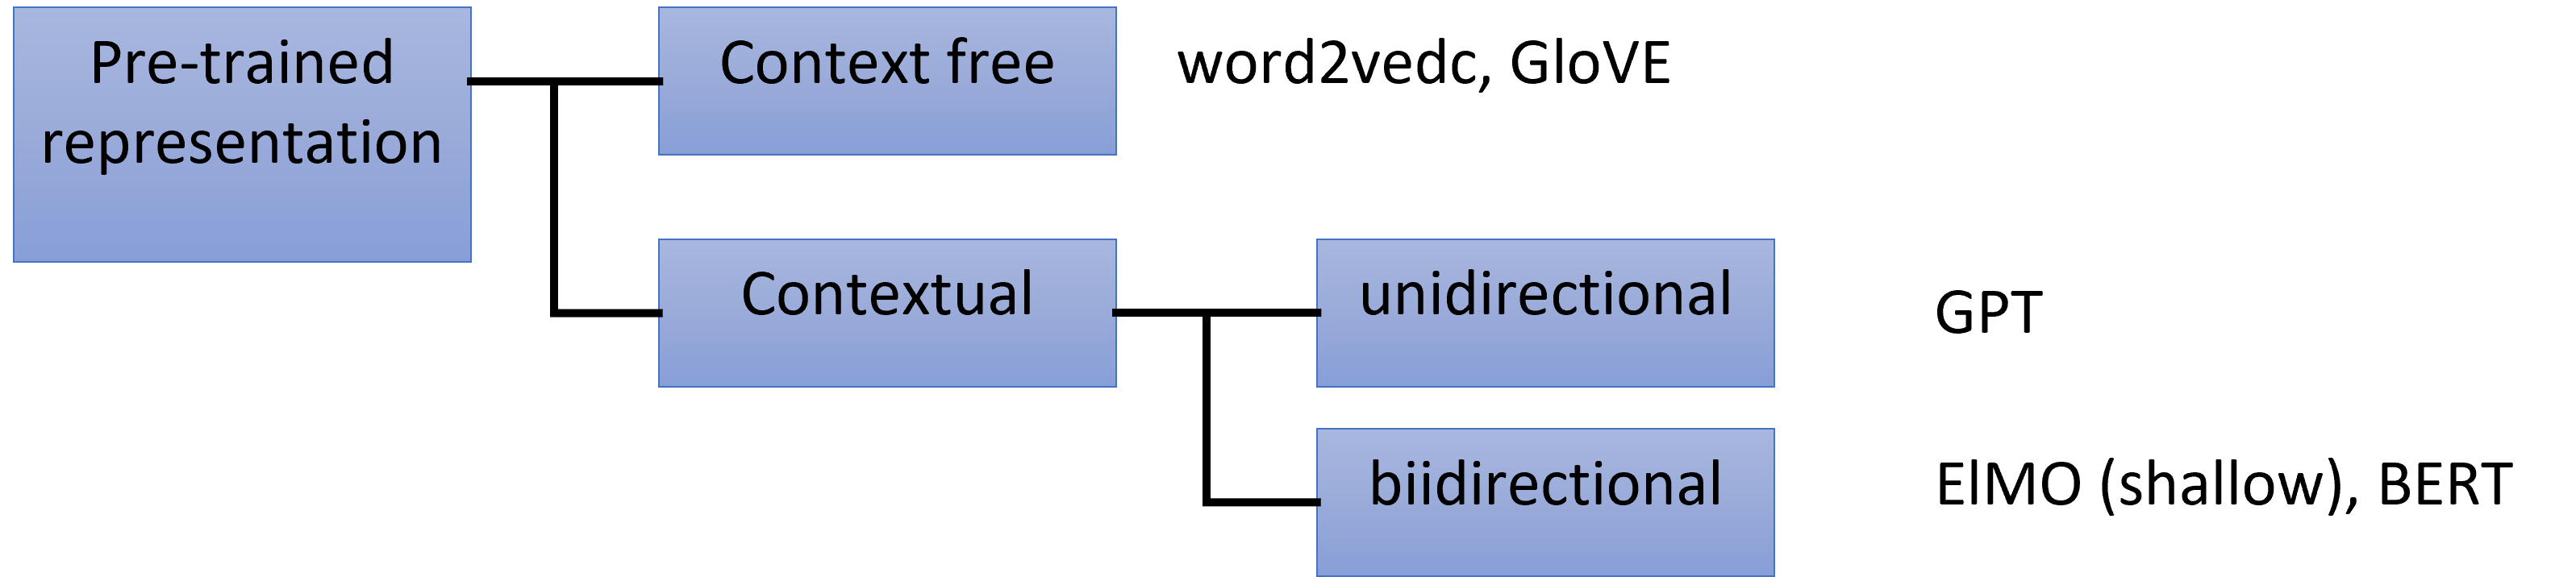
\includegraphics[width=\linewidth,keepaspectratio]{bert113}
			\end{center}		
			

\end{frame}

%%%%%%%%%%%%%%%%%%%%%%%%%%%%%%%%%%%%%%%%%%%%%%%%%%%%%%%%%%%
\begin{frame}[fragile]\frametitle{What is BERT?}


			\begin{center}
Bert stands for Bidirectional Encoder Representations from Transformers. It’s google’s new techniques for NLP pre-training language representation. Which means now machine learning communities can use Bert models that have been training already on a large number of words, for NLP models to do a wide variety of tasks such as Question Answering tasks, Named Entity Recognition (NER), and Classification like sentiment analysis.
			\end{center}		
			

\end{frame}

%%%%%%%%%%%%%%%%%%%%%%%%%%%%%%%%%%%%%%%%%%%%%%%%%%%%%%%%%%%
\begin{frame}[fragile]\frametitle{}

\begin{columns}
    \begin{column}[T]{0.5\linewidth}
			\begin{center}
			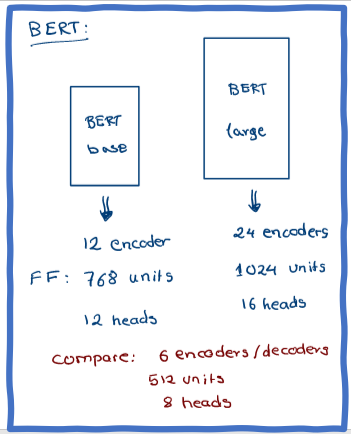
\includegraphics[width=0.8\linewidth,keepaspectratio]{bert114}
			\end{center}		
		\end{column}
    \begin{column}[T]{0.5\linewidth}
In Bert paper, they present two types of Bert models one is the Bert Base and the other is Bert Large.

    \end{column}
  \end{columns}
			
\end{frame}

%%%%%%%%%%%%%%%%%%%%%%%%%%%%%%%%%%%%%%%%%%%%%%%%%%%%%%%%%%%
\begin{frame}[fragile]\frametitle{}


			\begin{center}
			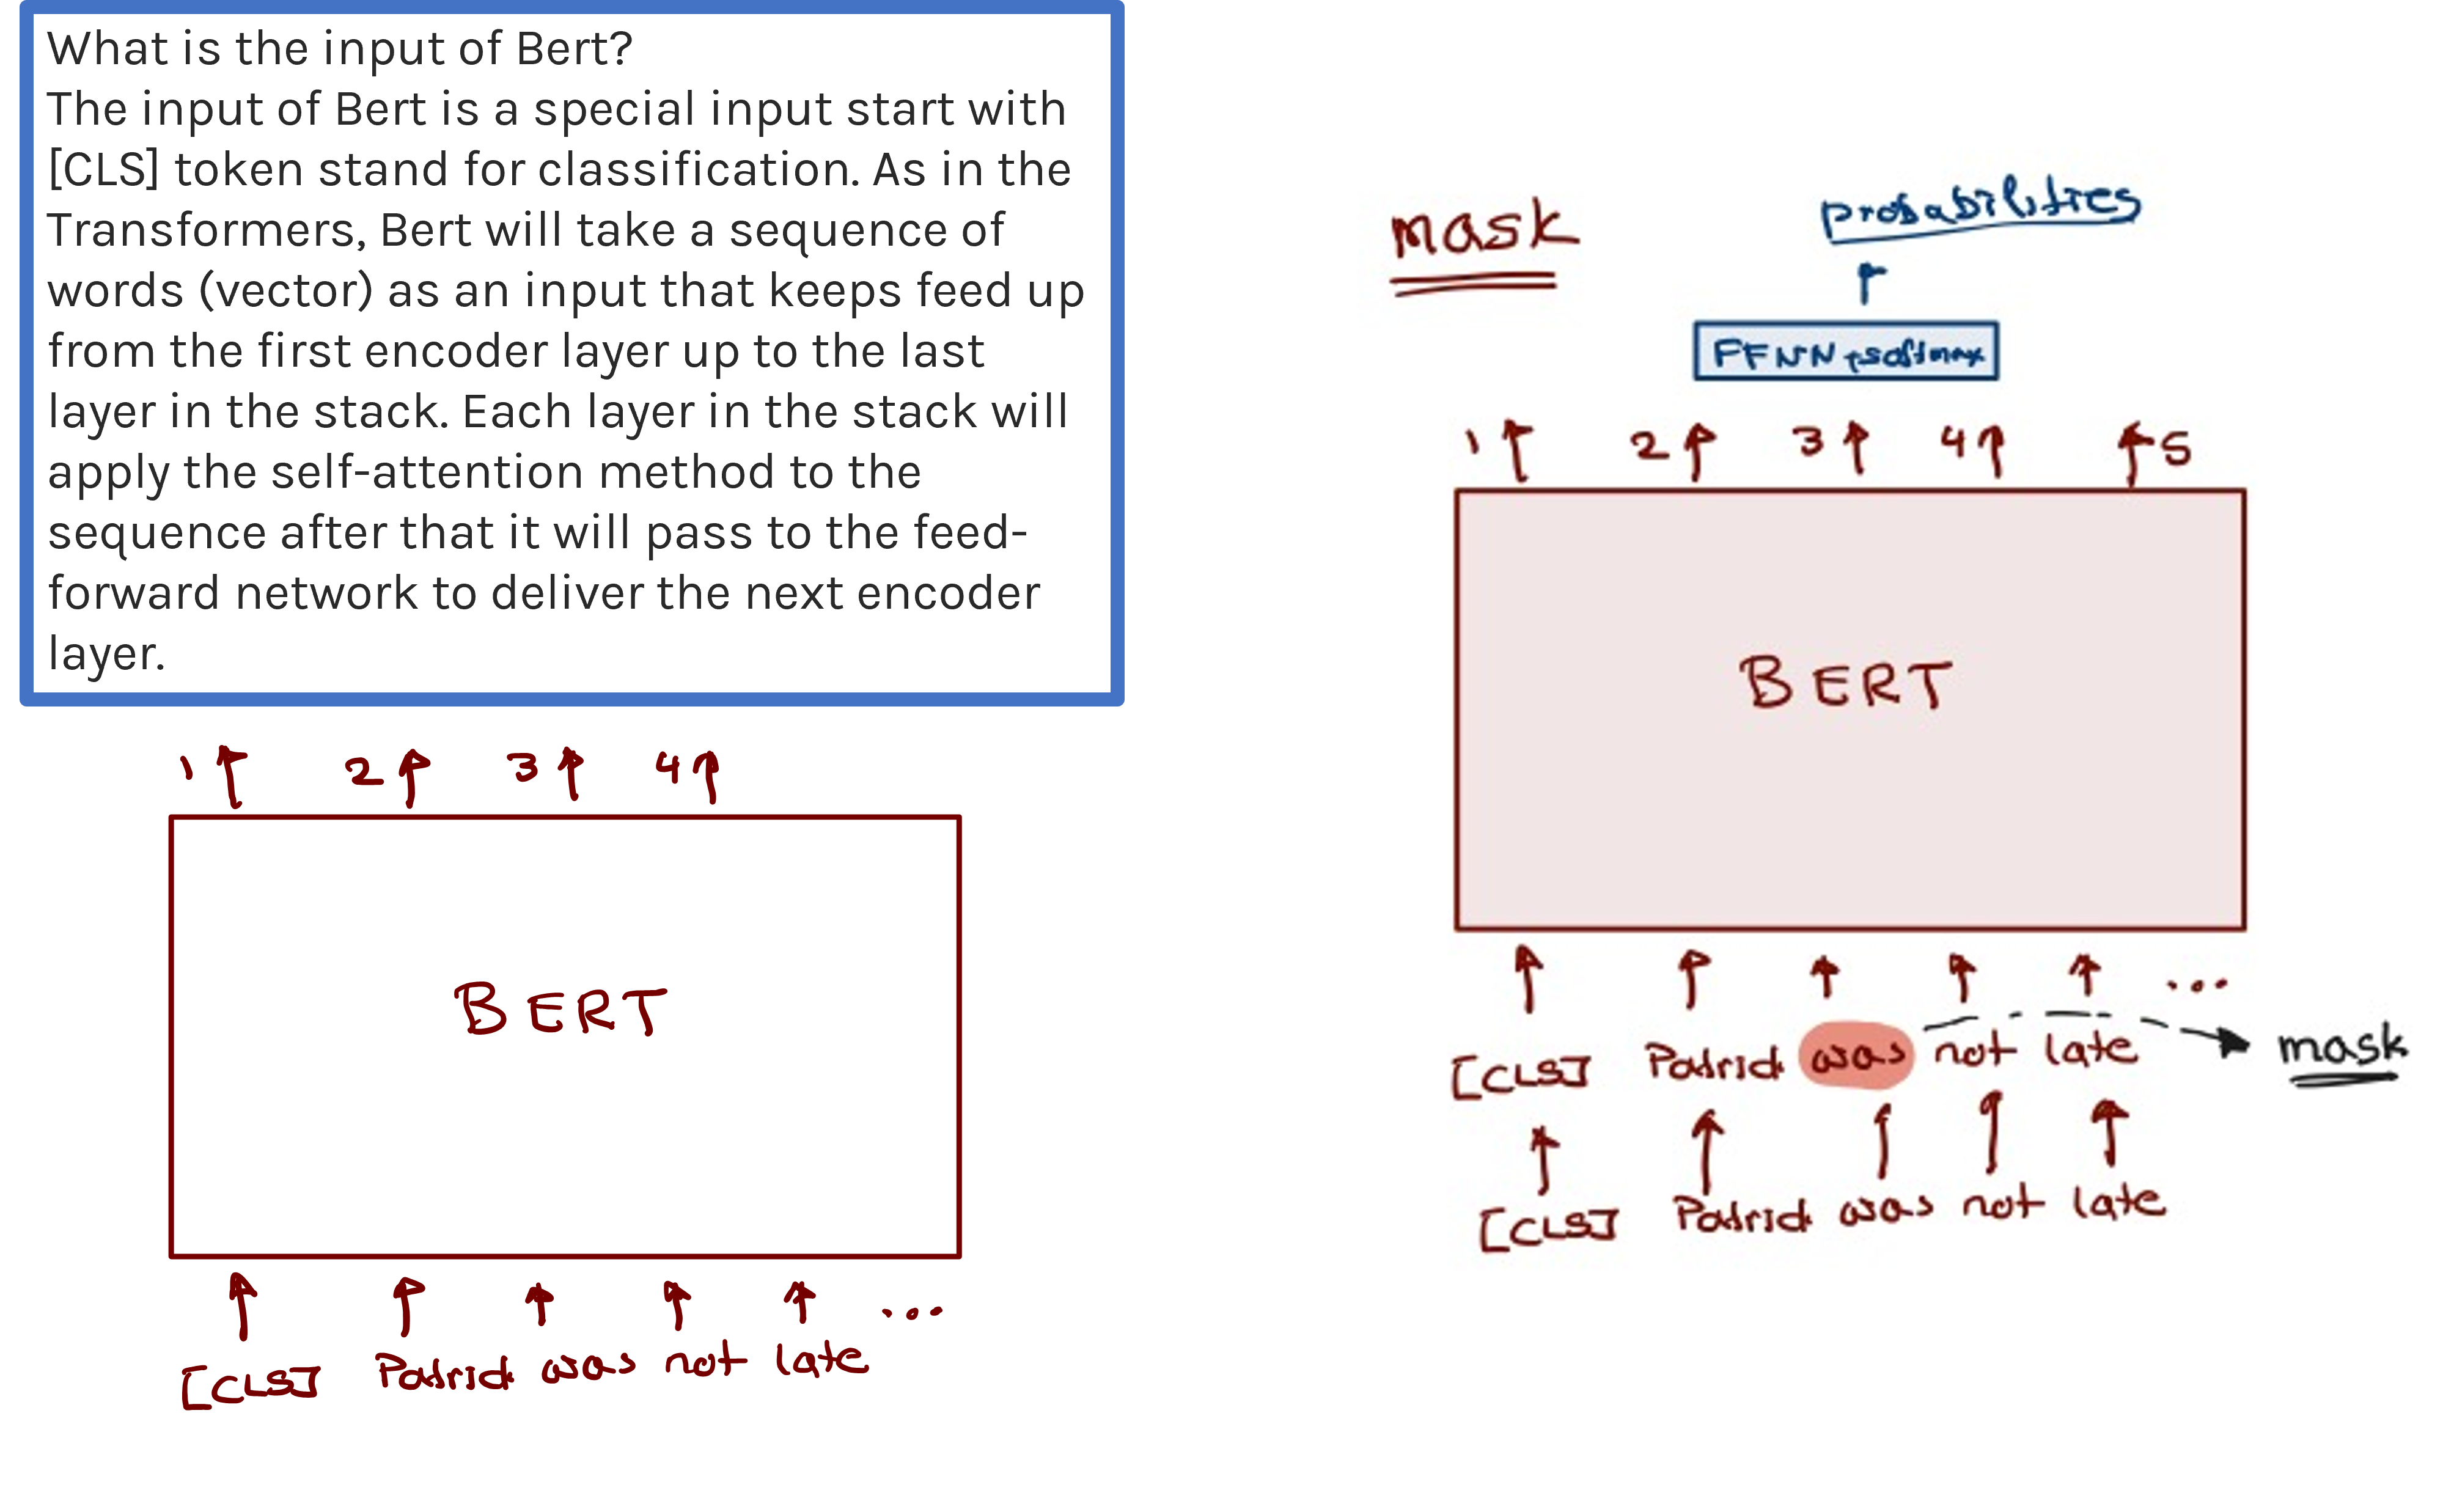
\includegraphics[width=\linewidth,keepaspectratio]{bert115}
			\end{center}		
			

\end{frame}

%%%%%%%%%%%%%%%%%%%%%%%%%%%%%%%%%%%%%%%%%%%%%%%%%%%%%%%%%%%
\begin{frame}[fragile]\frametitle{}


			\begin{center}
			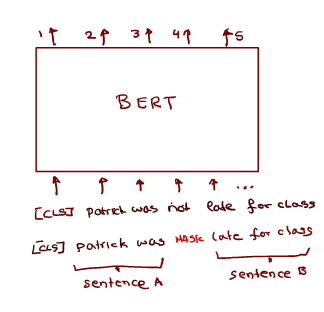
\includegraphics[width=0.5\linewidth,keepaspectratio]{bert116}
			\end{center}		
			

\end{frame}

% %%%%%%%%%%%%%%%%%%%%%%%%%%%%%%%%%%%%%%%%%%%%%%%%%%%%%%%%%%%
% \begin{frame}[fragile]\frametitle{}

			% \begin{center}
			% 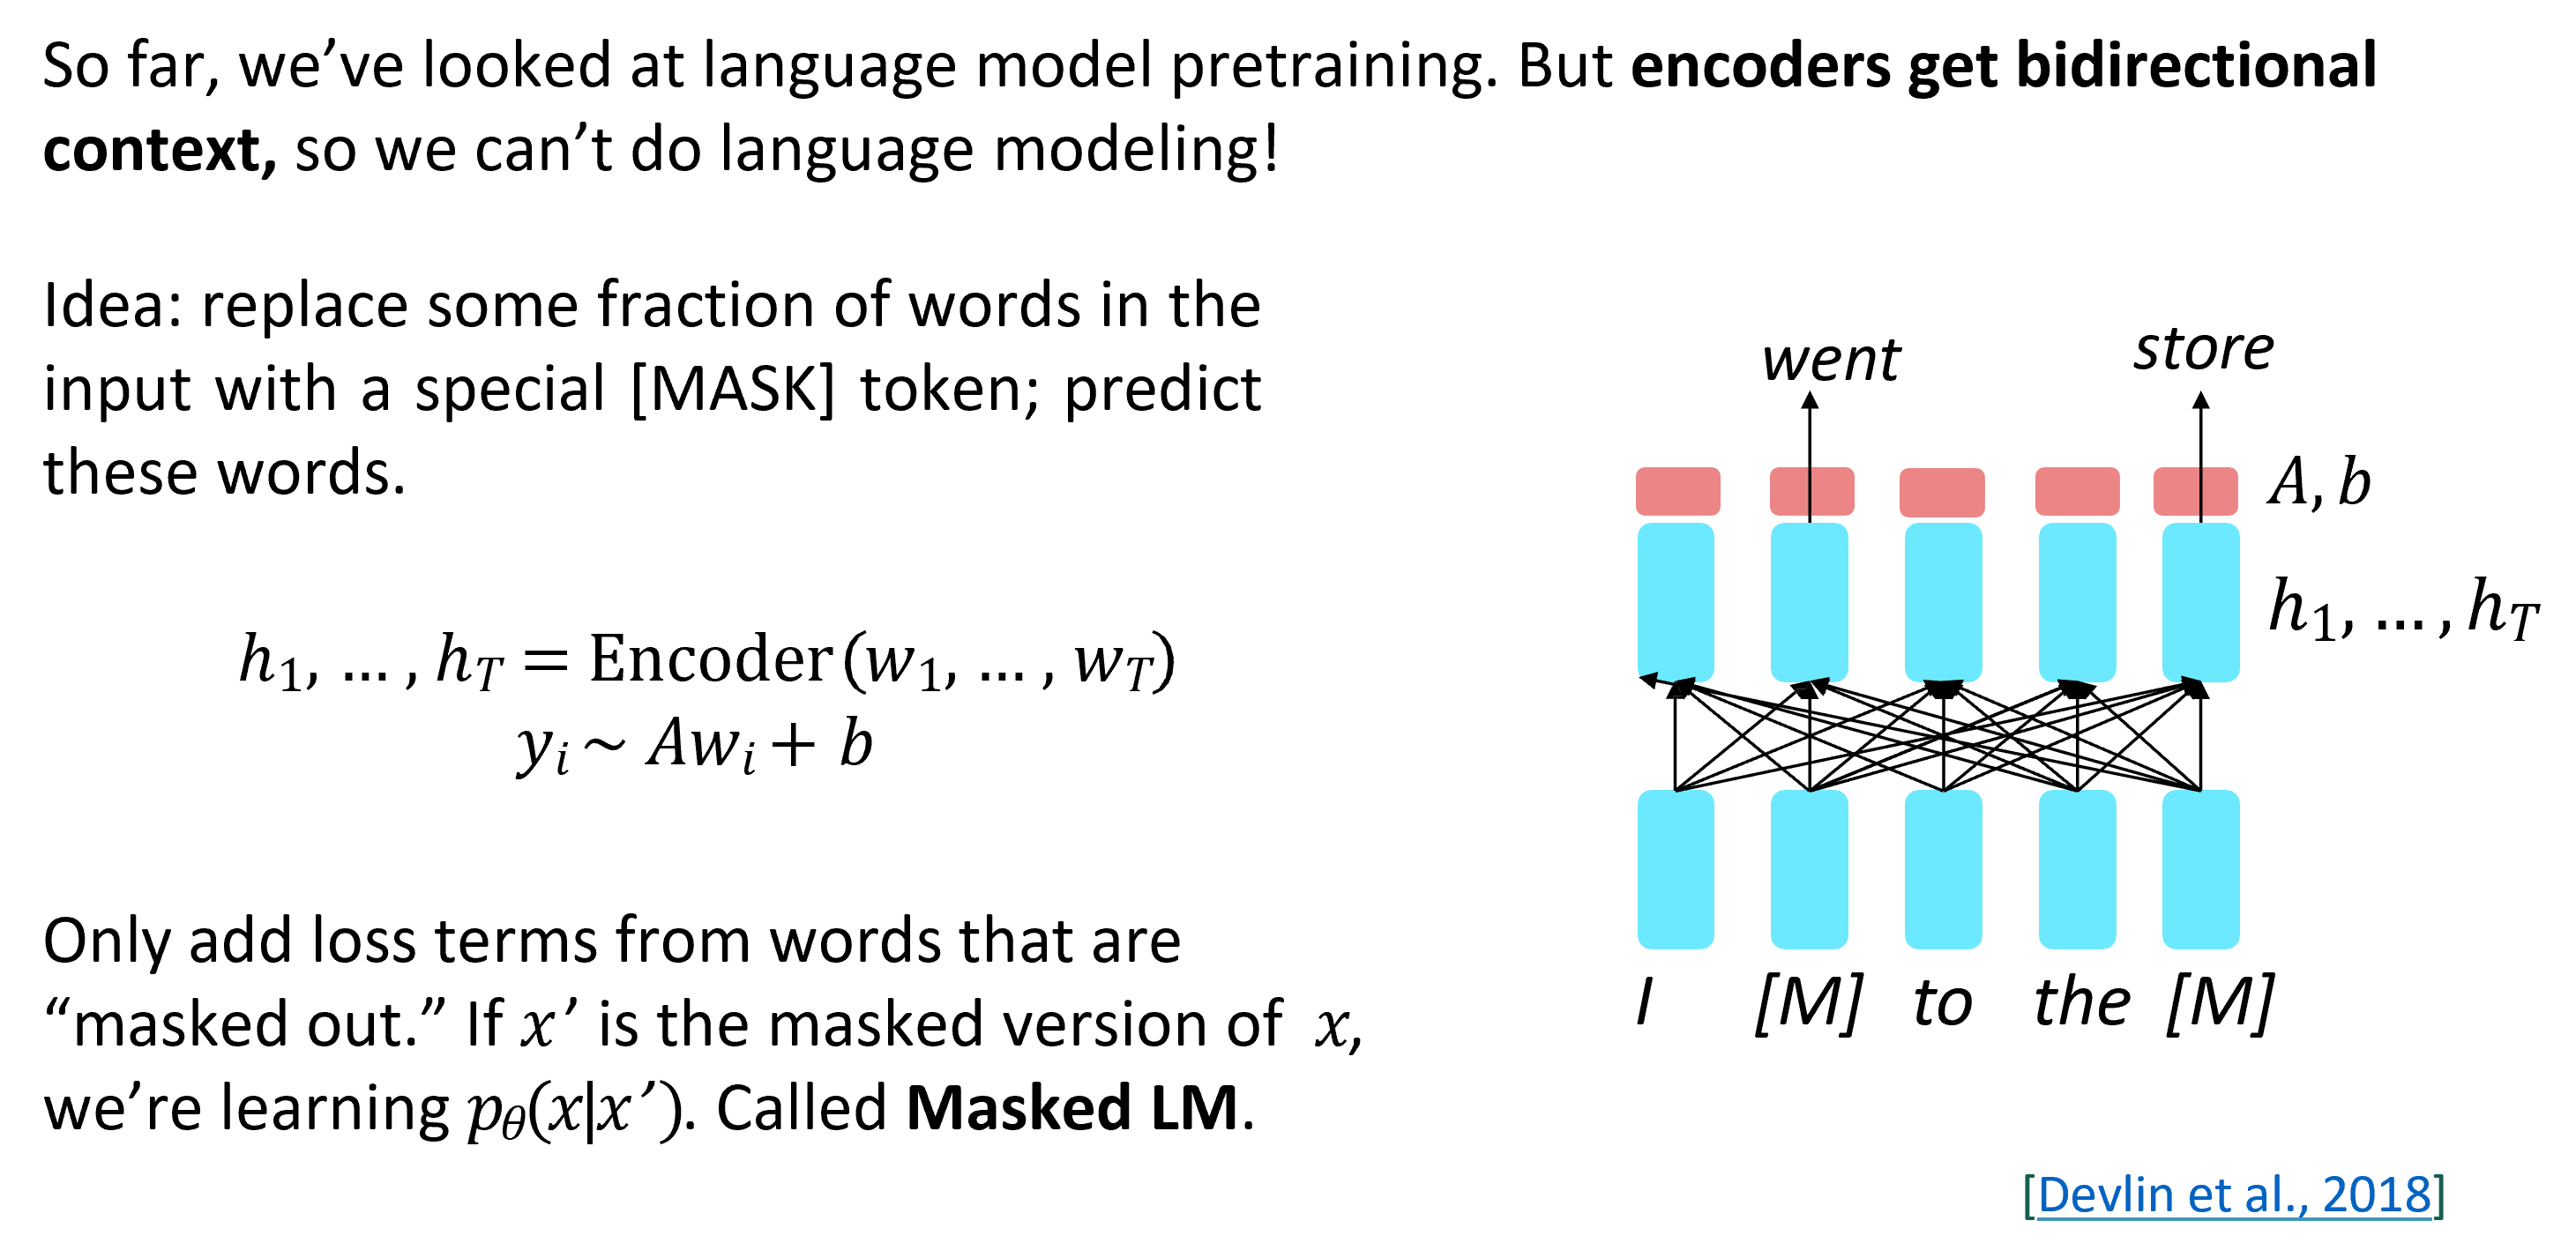
\includegraphics[width=\linewidth,keepaspectratio]{bert117}
			% \end{center}		
			
% \end{frame}

% %%%%%%%%%%%%%%%%%%%%%%%%%%%%%%%%%%%%%%%%%%%%%%%%%%%%%%%%%%%
% \begin{frame}[fragile]\frametitle{Pretraining encoders: What pretraining objective to use?}

			% \begin{center}
			% 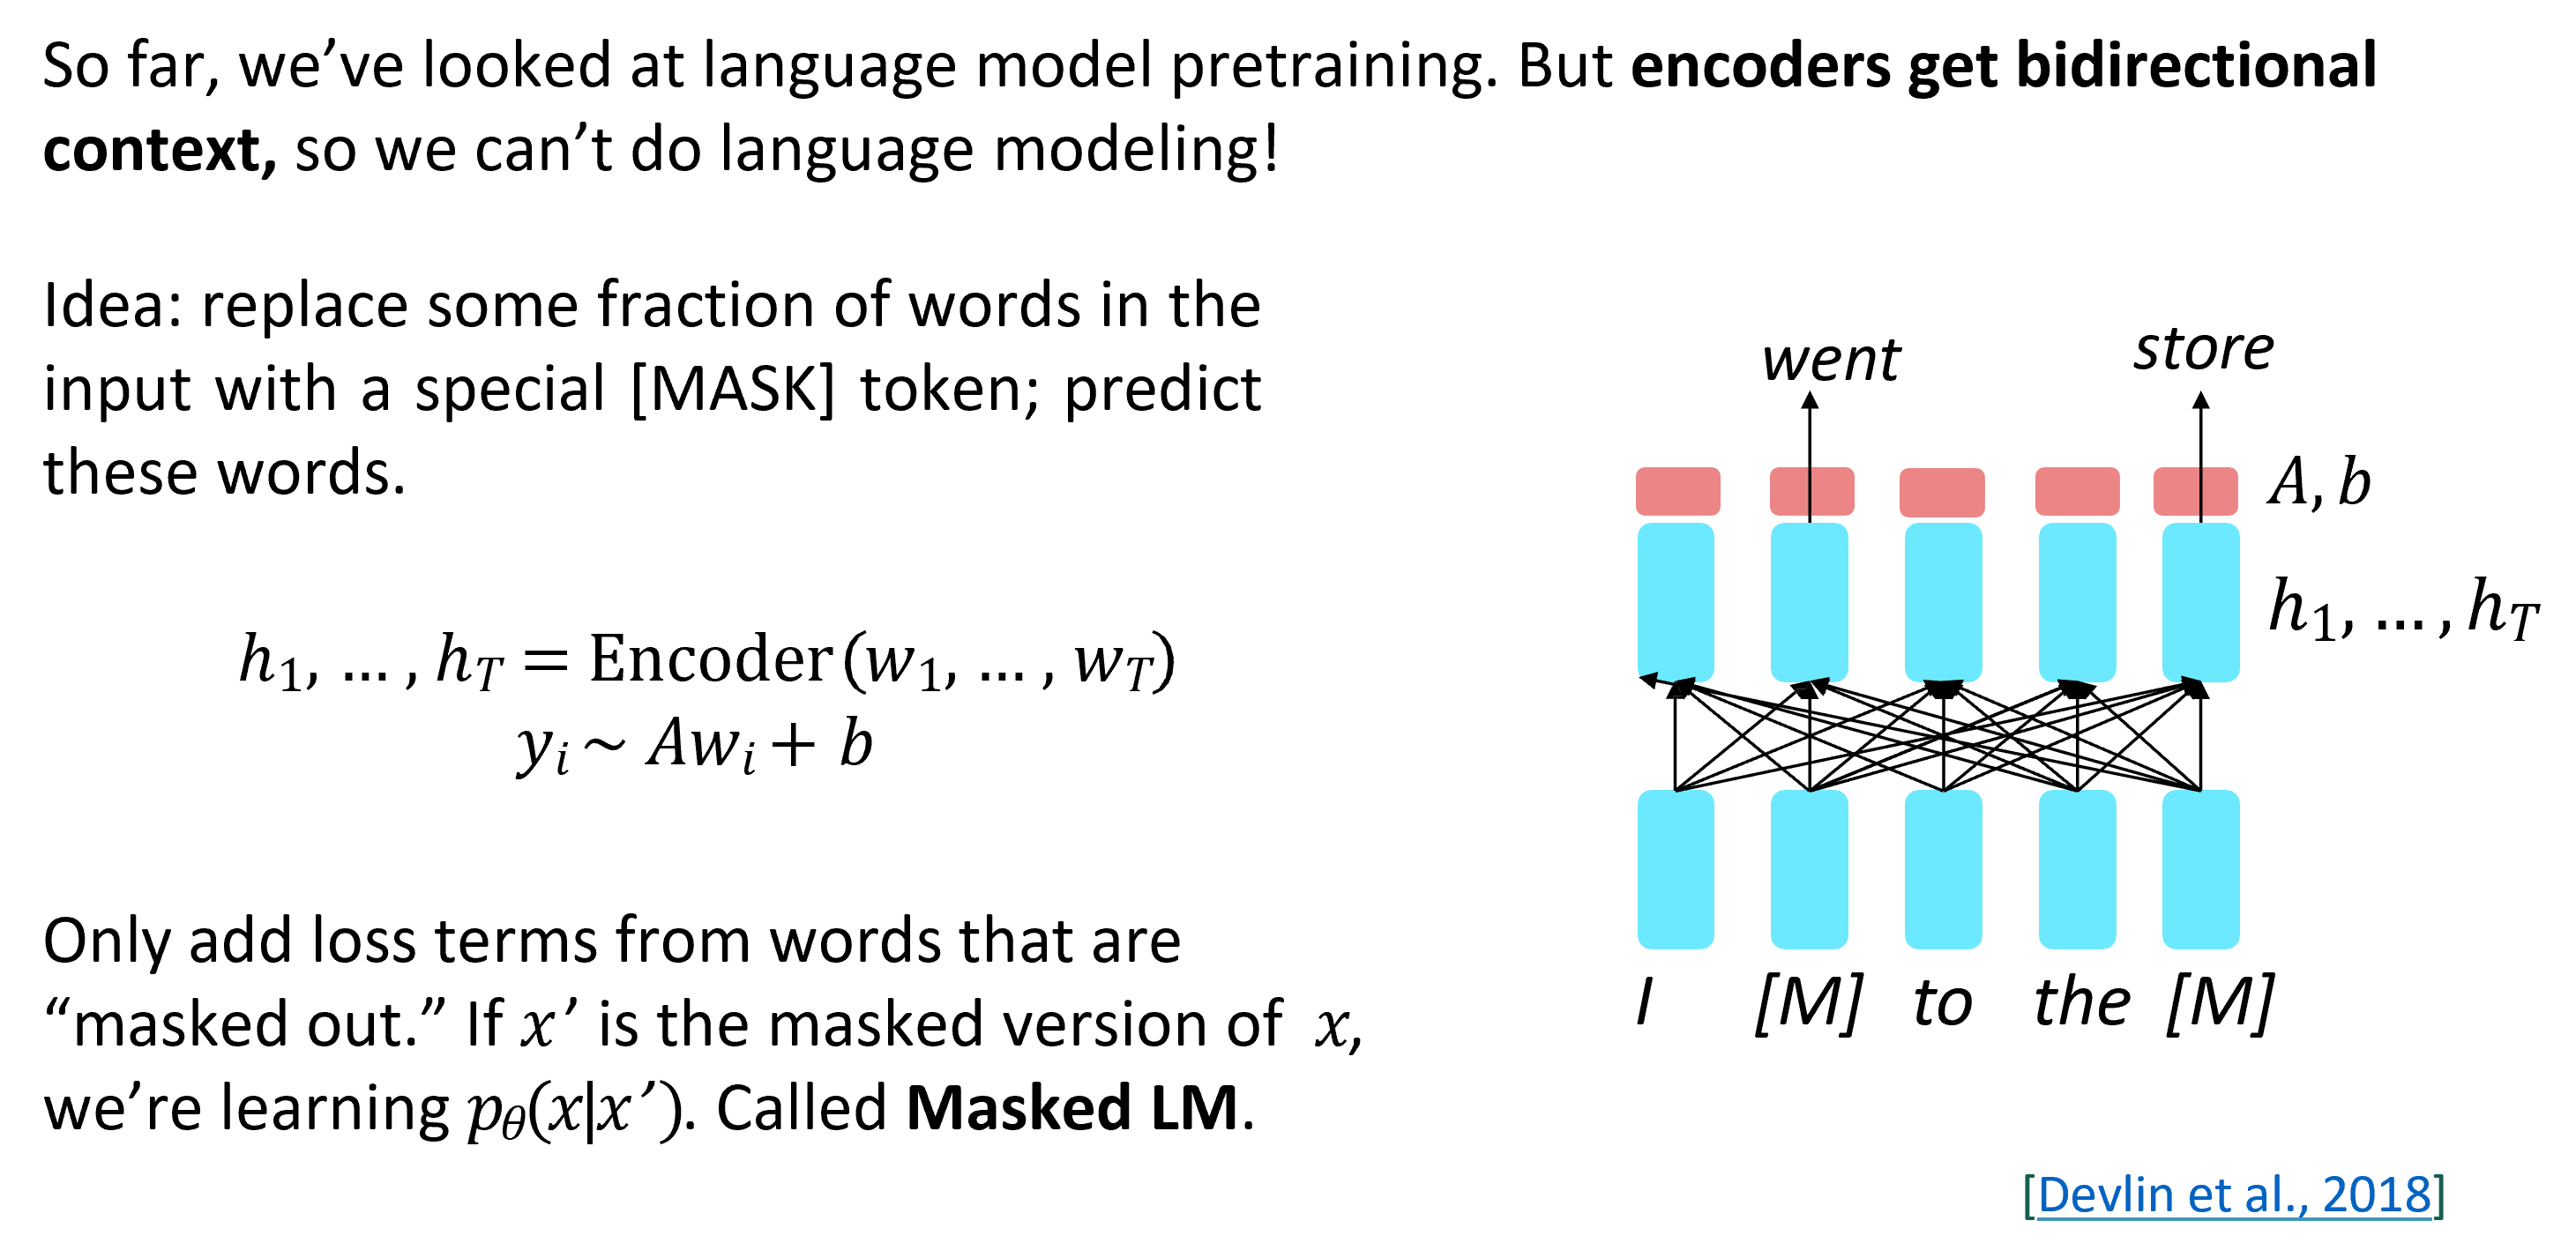
\includegraphics[width=\linewidth,keepaspectratio]{bert118}
			% \end{center}		
			
			% % {\tiny (Ref: John Hewitt)}

% \end{frame}

%%%%%%%%%%%%%%%%%%%%%%%%%%%%%%%%%%%%%%%%%%%%%%%%%%%%%%%%%%%
\begin{frame}[fragile]\frametitle{BERT: Bidirectional Encoder Representations from Transformers}

			\begin{center}
			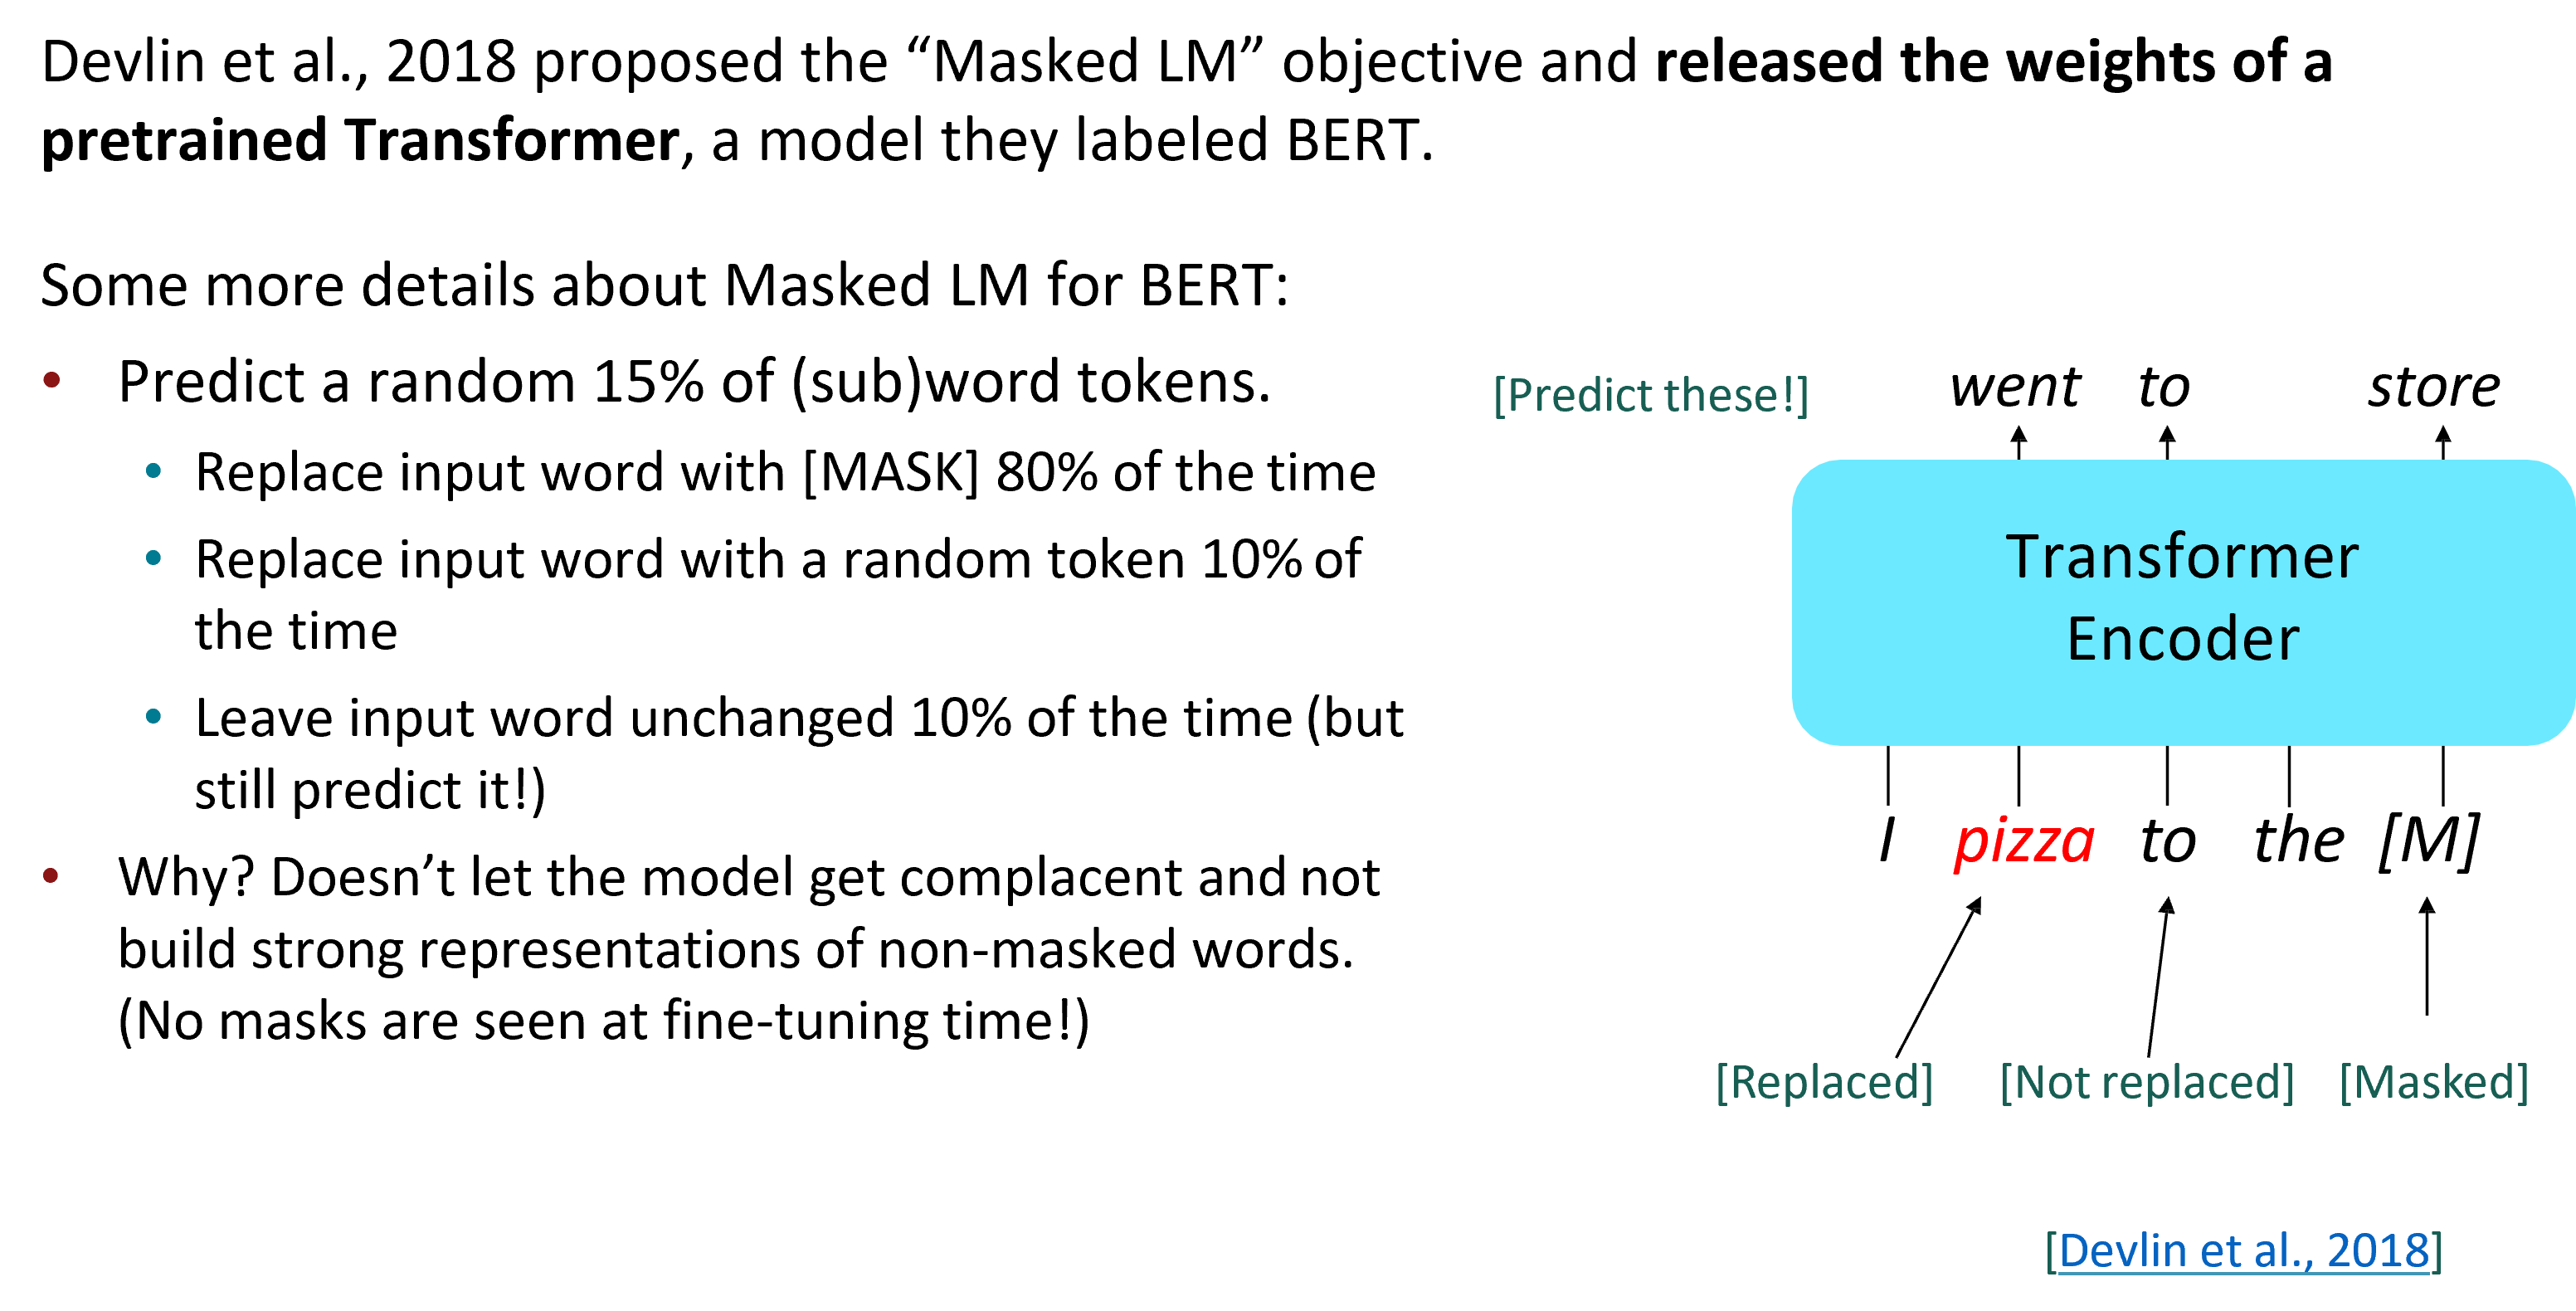
\includegraphics[width=\linewidth,keepaspectratio]{bert119}
			\end{center}		
			
% {\tiny (Ref: CS224n: Natural Language Processing with Deep Learning - Christopher Manning)}

\end{frame}

%%%%%%%%%%%%%%%%%%%%%%%%%%%%%%%%%%%%%%%%%%%%%%%%%%%%%%%%%%%
\begin{frame}[fragile]\frametitle{BERT: Bidirectional Encoder Representations from Transformers}

			\begin{center}
			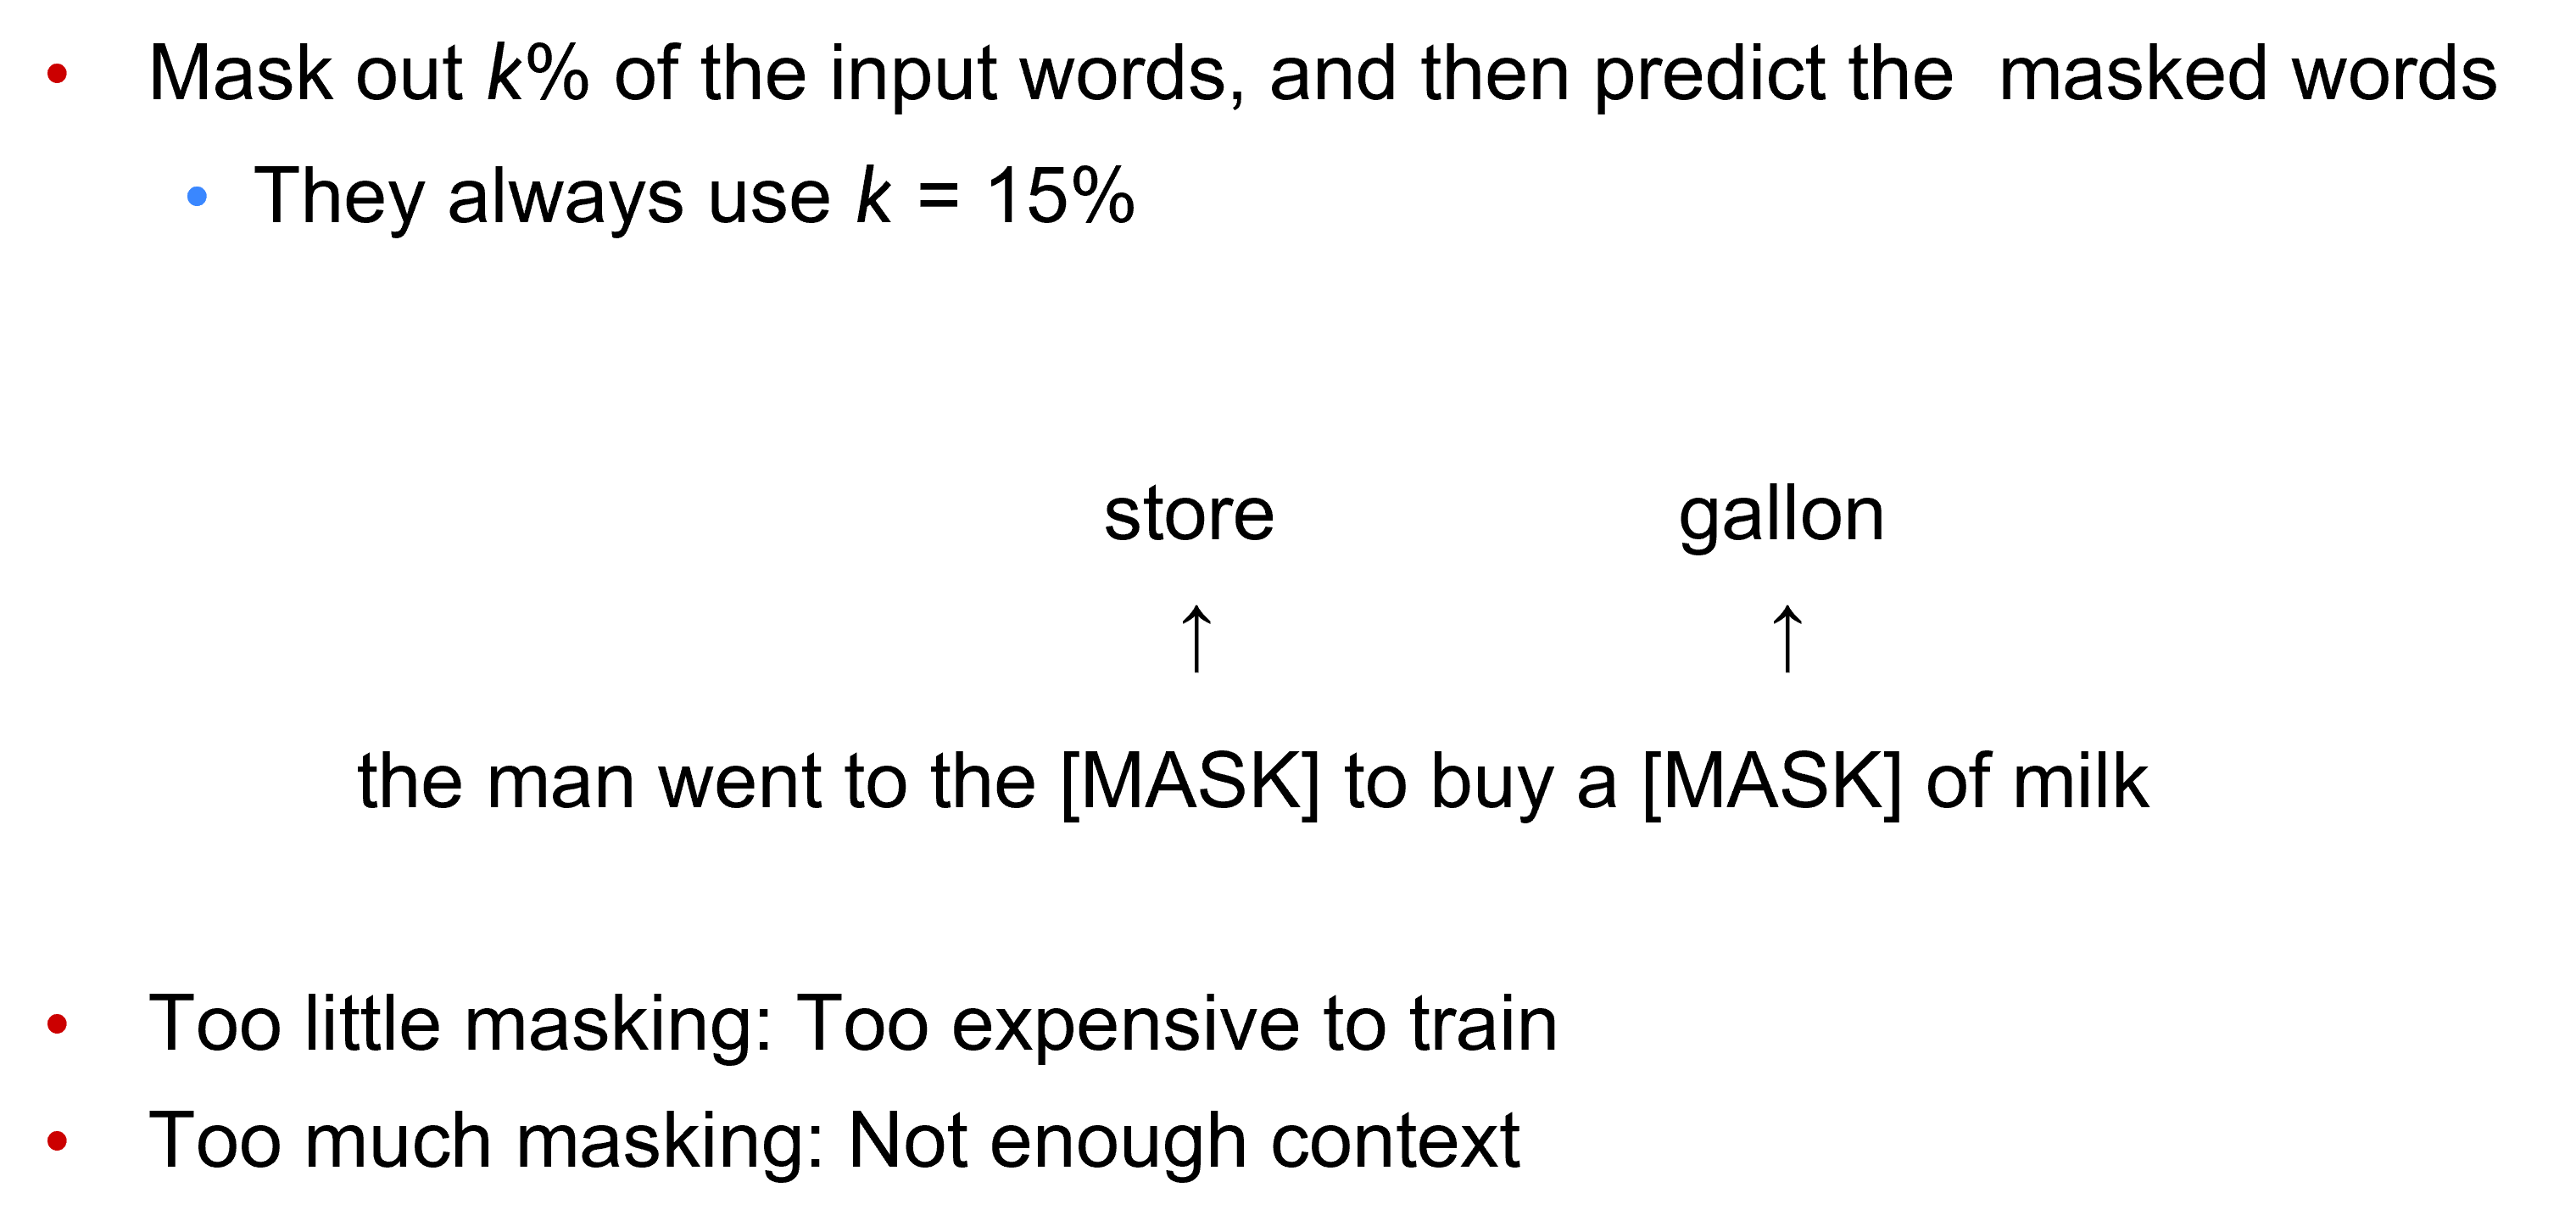
\includegraphics[width=0.8\linewidth,keepaspectratio]{bert120}
			\end{center}		
			
% {\tiny (Ref: CS224n: Natural Language Processing with Deep Learning - Christopher Manning)}

\end{frame}

%%%%%%%%%%%%%%%%%%%%%%%%%%%%%%%%%%%%%%%%%%%%%%%%%%%%%%%%%%%
\begin{frame}[fragile]\frametitle{BERT: Bidirectional Encoder Representations from Transformers}

			\begin{center}
			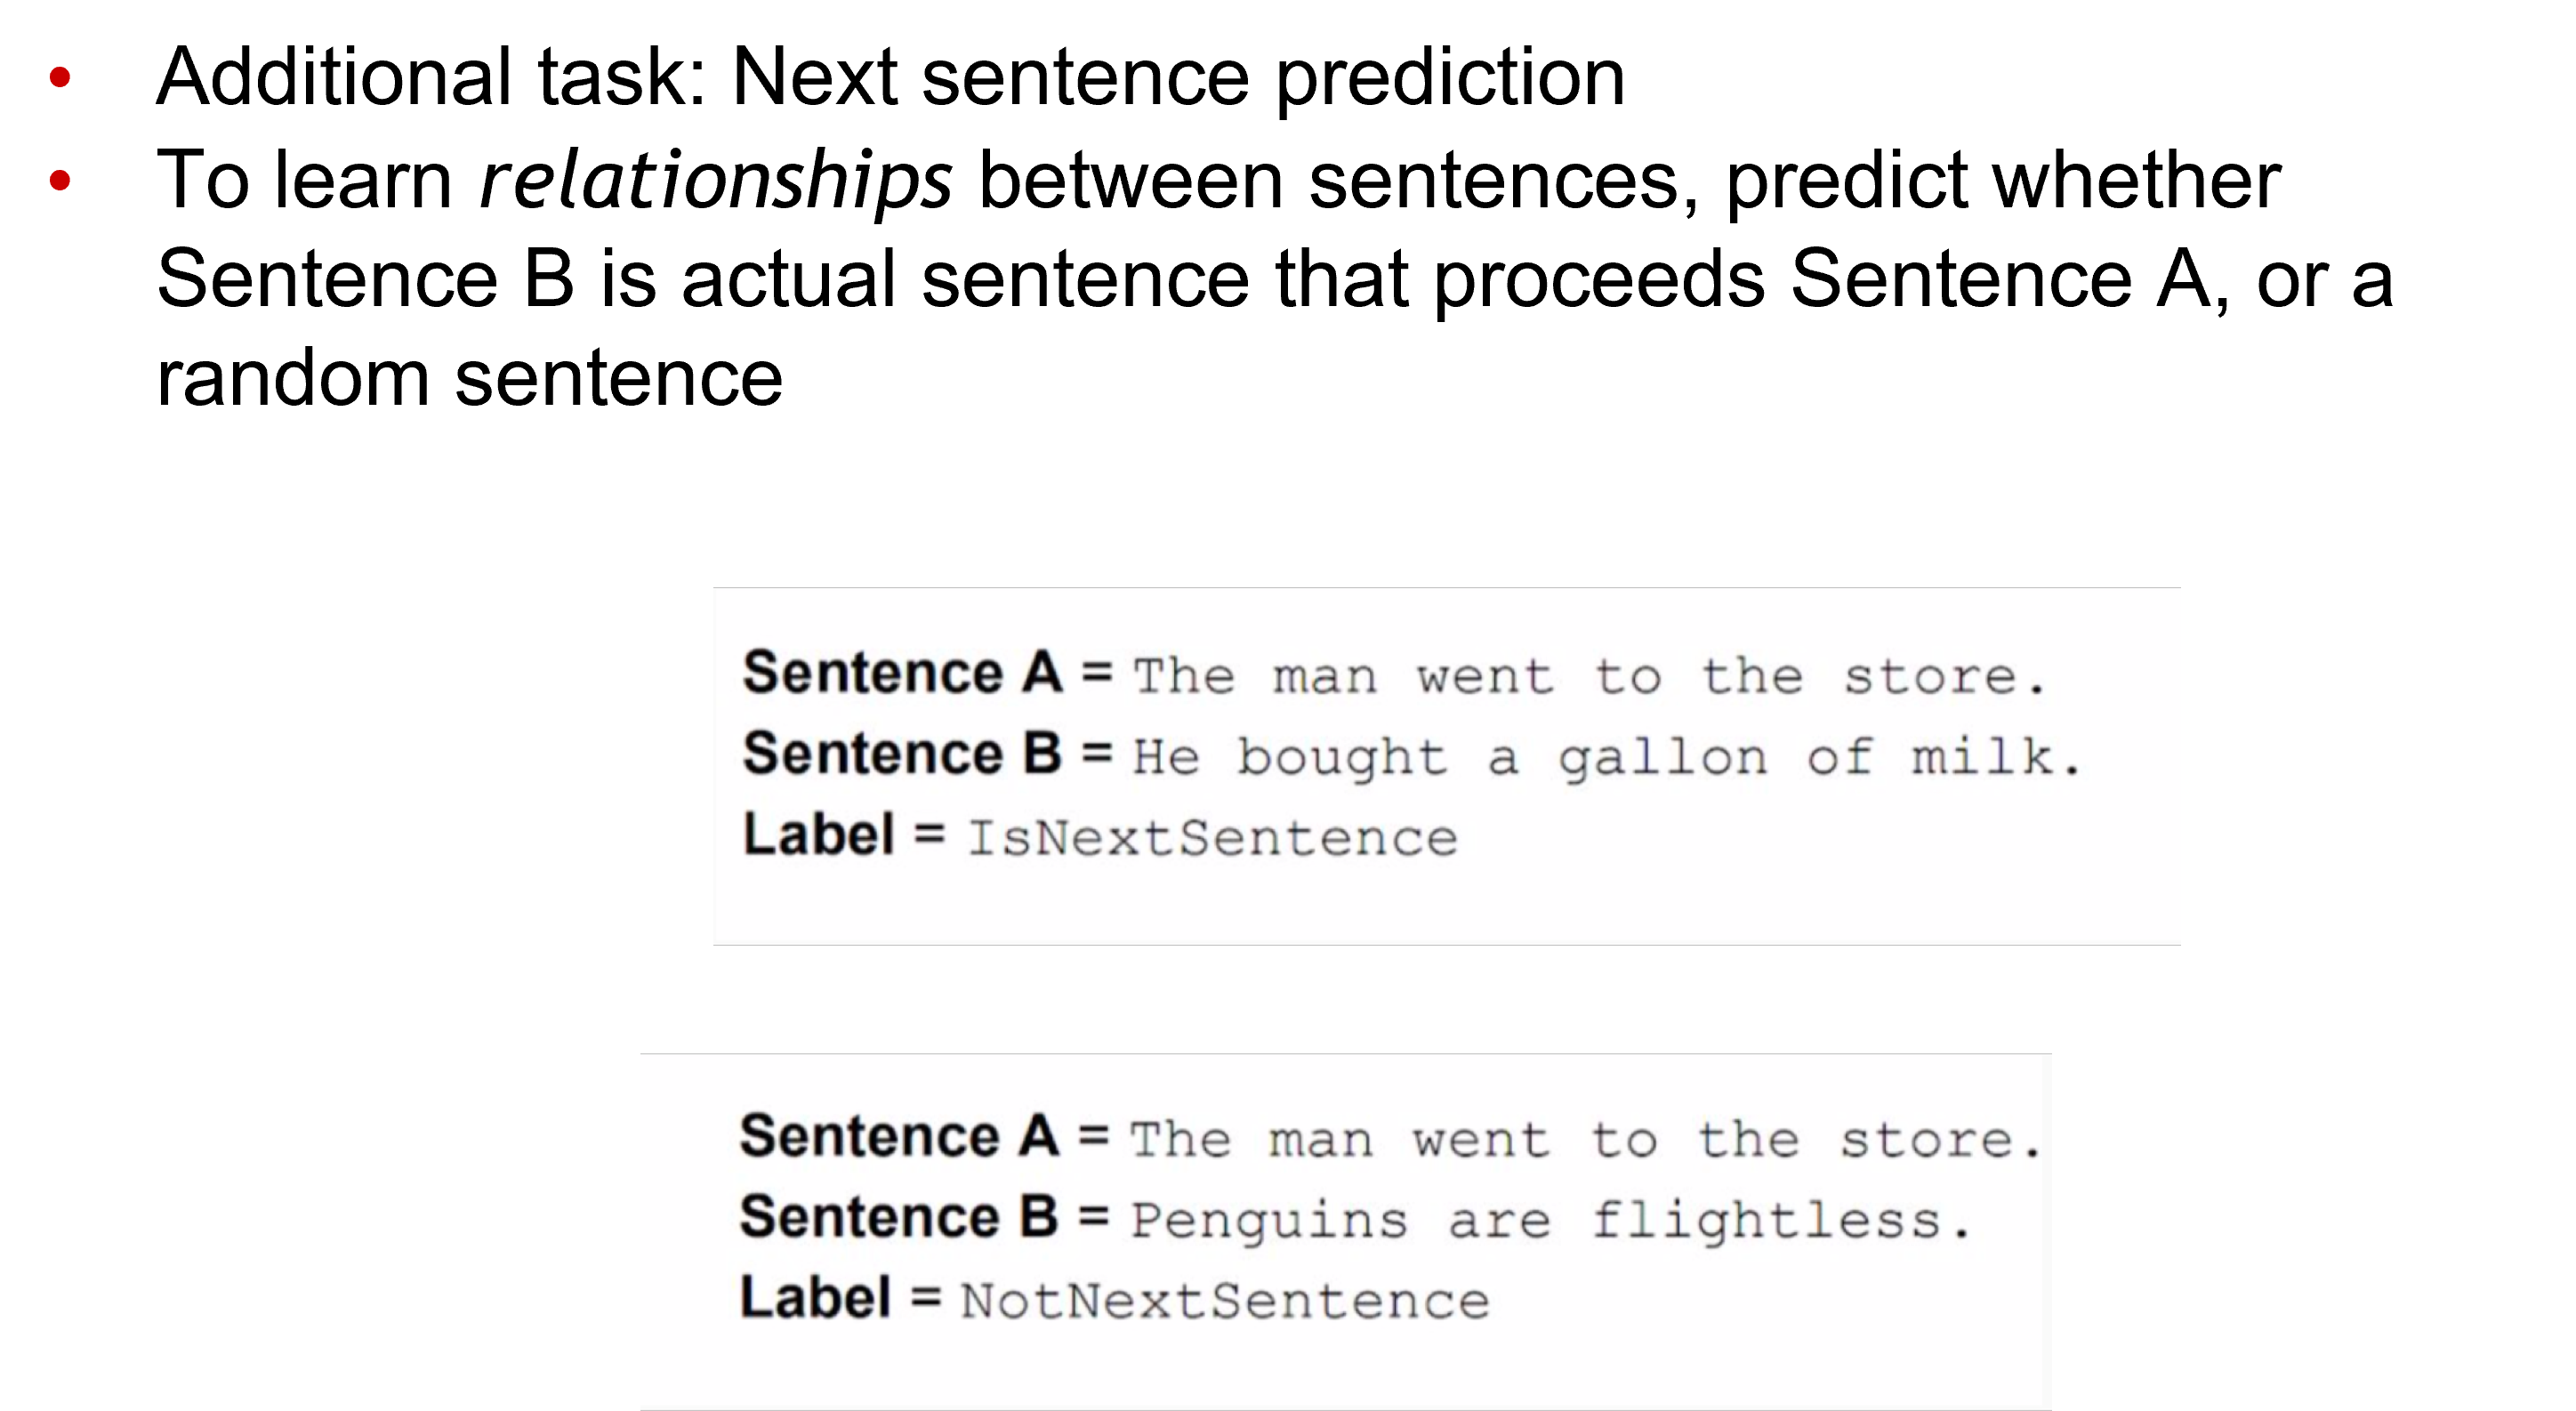
\includegraphics[width=\linewidth,keepaspectratio]{bert121}
			\end{center}		
			
% {\tiny (Ref: CS224n: Natural Language Processing with Deep Learning - Christopher Manning)}

\end{frame}

%%%%%%%%%%%%%%%%%%%%%%%%%%%%%%%%%%%%%%%%%%%%%%%%%%%%%%%%%%%
\begin{frame}[fragile]\frametitle{BERT: Bidirectional Encoder Representations from Transformers}

			\begin{center}
			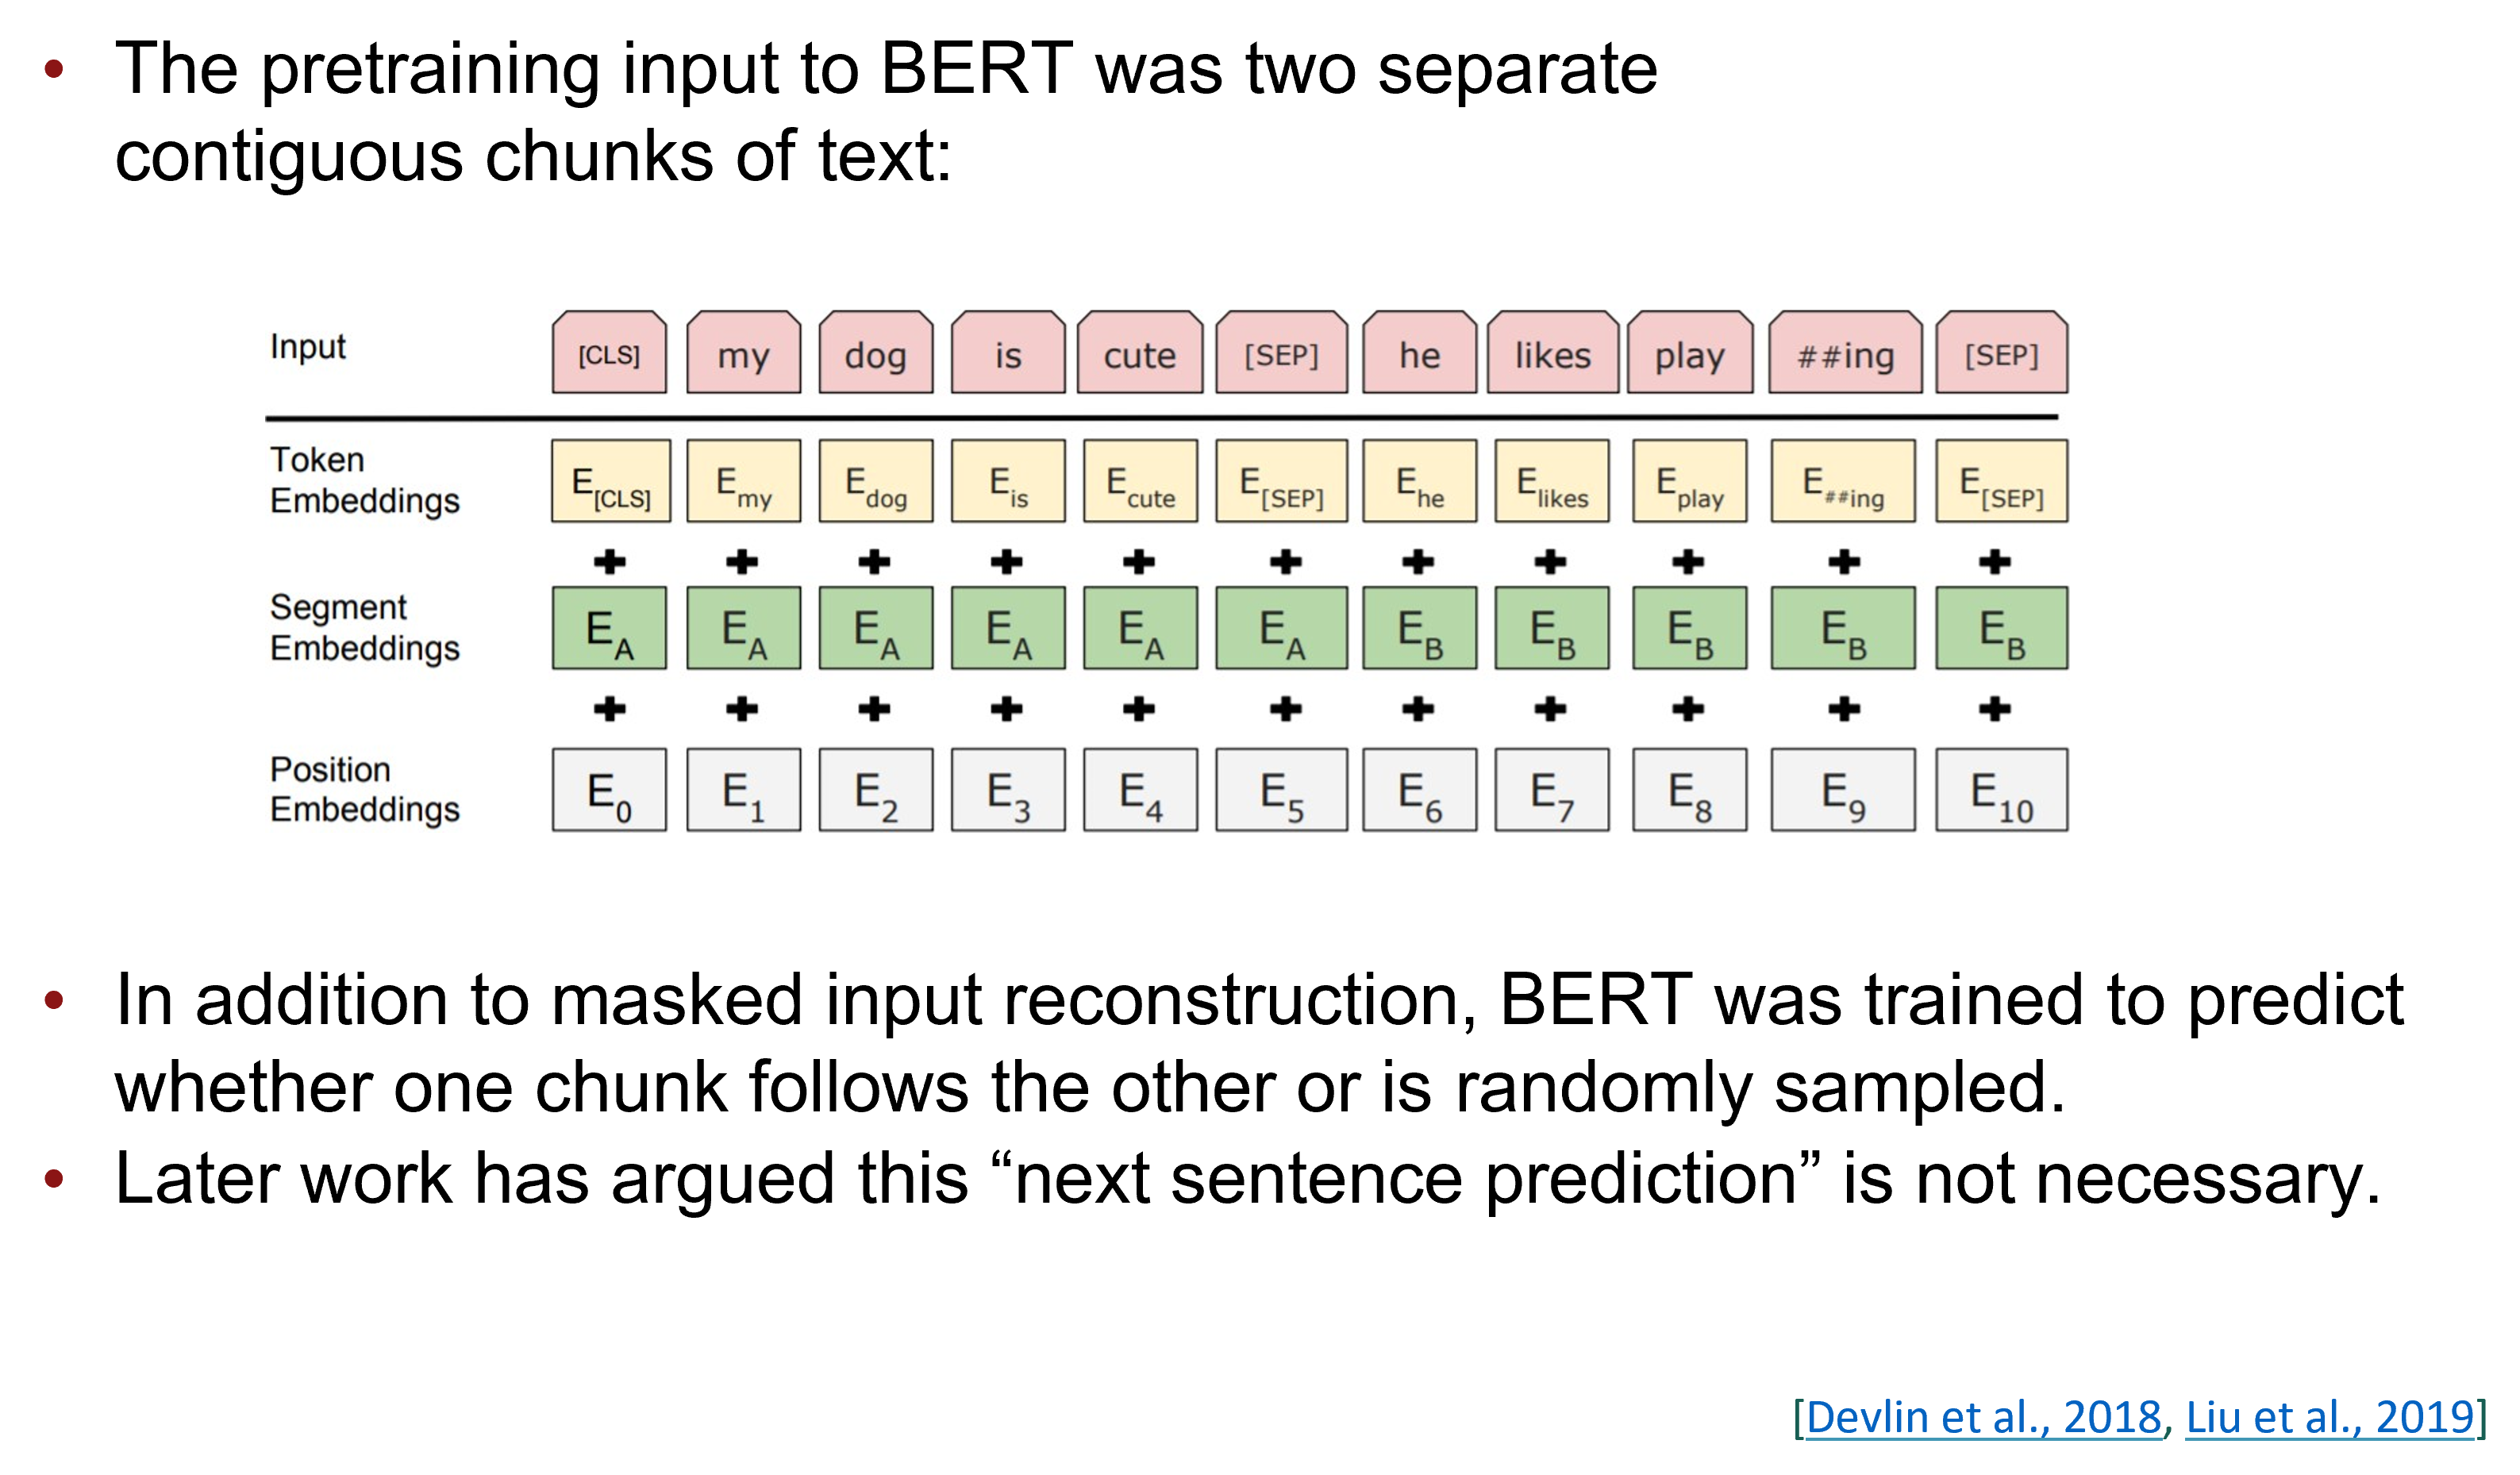
\includegraphics[width=\linewidth,keepaspectratio]{bert122}
			\end{center}		
			
% {\tiny (Ref: CS224n: Natural Language Processing with Deep Learning - Christopher Manning)}

\end{frame}

%%%%%%%%%%%%%%%%%%%%%%%%%%%%%%%%%%%%%%%%%%%%%%%%%%%%%%%%%%%
\begin{frame}[fragile]\frametitle{BERT: Bidirectional Encoder Representations from Transformers}

Details about BERT


      \begin{itemize}
			\item Two models were released:
			      \begin{itemize}
						\item BERT-base: 12 layers, 768-dim hidden states, 12 attention heads, 110 million params.
						\item BERT-large: 24 layers, 1024-dim hidden states, 16 attention heads, 340 million params.
						\end{itemize}

			\item Trained on:
			      \begin{itemize}
						\item BooksCorpus (800 million words)
						\item English Wikipedia (2,500 million words)
						\end{itemize}

			\item Pretraining is expensive and impractical on a single GPU.
			      \begin{itemize}
						\item BERT was pretrained with 64 TPU chips for a total of 4 days.
						\item (TPUs are special tensor operation acceleration hardware)
						\end{itemize}

			\item Finetuning is practical and common on a single GPU
			      \begin{itemize}
						\item ``Pretrain once, finetune many times.''
						\end{itemize}

			\end{itemize}
			
% {\tiny (Ref: CS224n: Natural Language Processing with Deep Learning - Christopher Manning)}

\end{frame}

%%%%%%%%%%%%%%%%%%%%%%%%%%%%%%%%%%%%%%%%%%%%%%%%%%%%%%%%%%%
\begin{frame}[fragile]\frametitle{BERT: Bidirectional Encoder Representations from Transformers}

			\begin{center}
			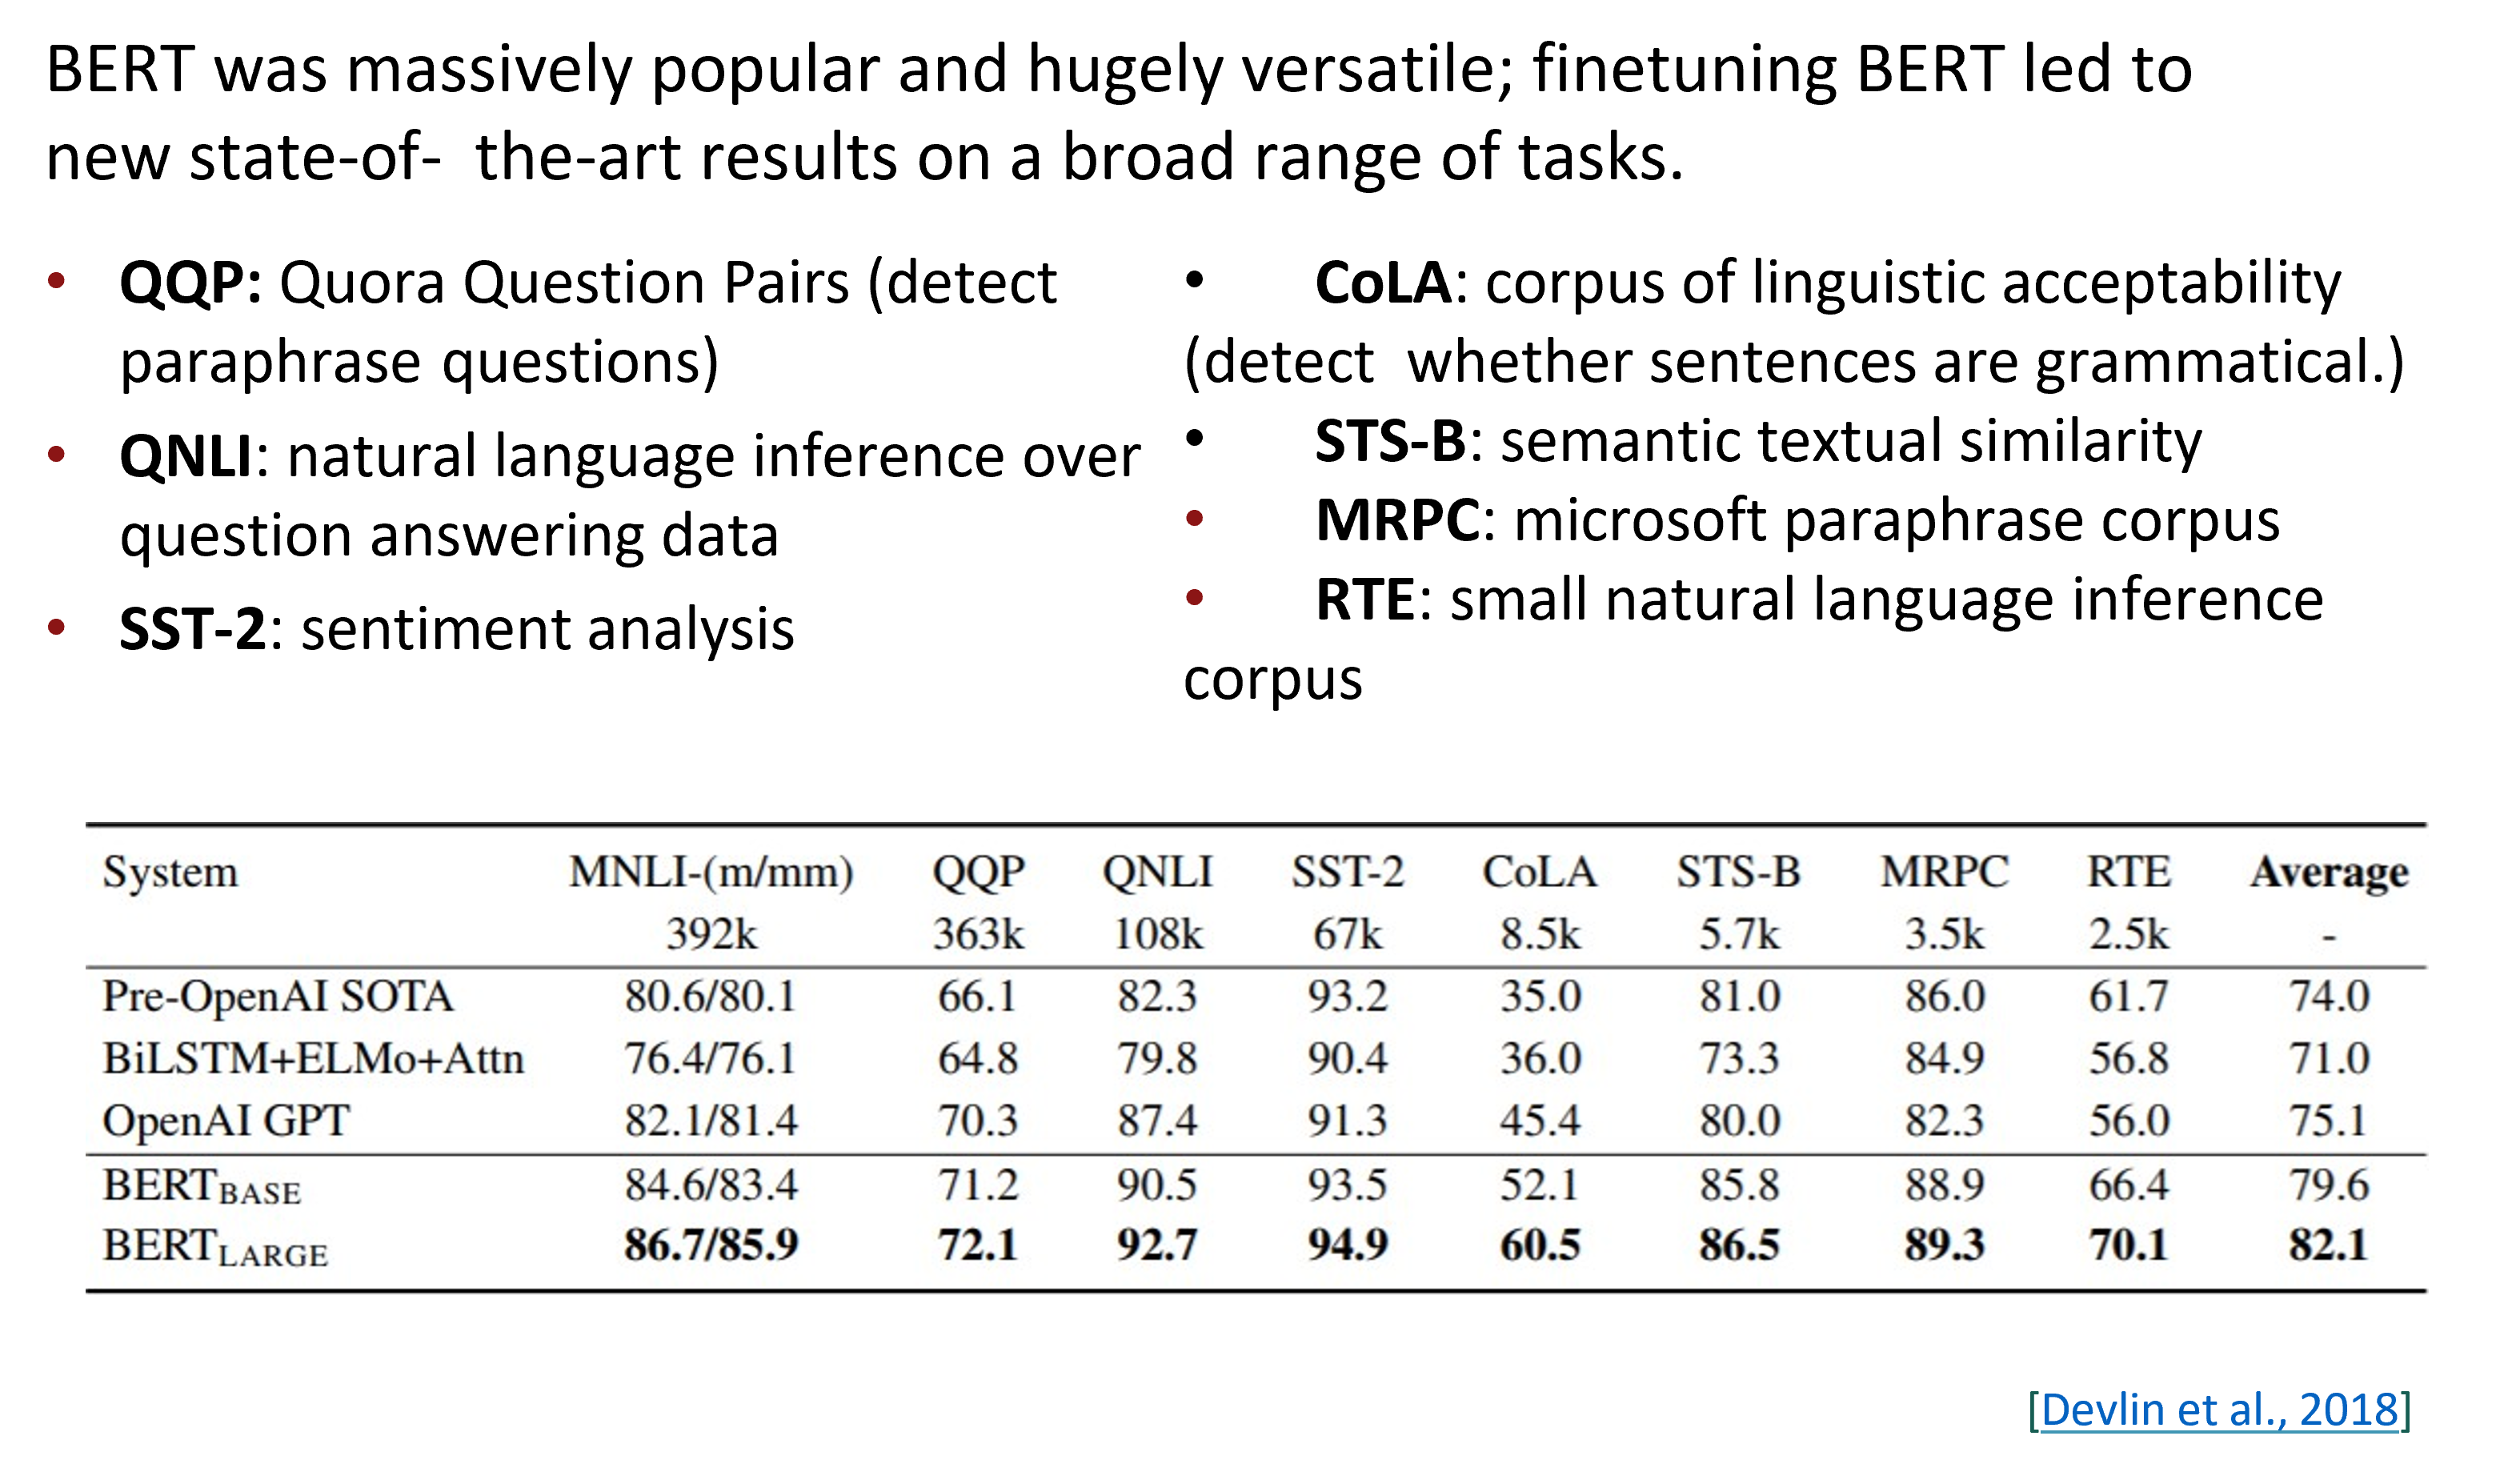
\includegraphics[width=\linewidth,keepaspectratio]{bert123}
			\end{center}		
			
			% {\tiny (Ref: John Hewitt)}

\end{frame}

%%%%%%%%%%%%%%%%%%%%%%%%%%%%%%%%%%%%%%%%%%%%%%%%%%%%%%%%%%%
\begin{frame}[fragile]\frametitle{Extensions of BERT}

			\begin{center}
			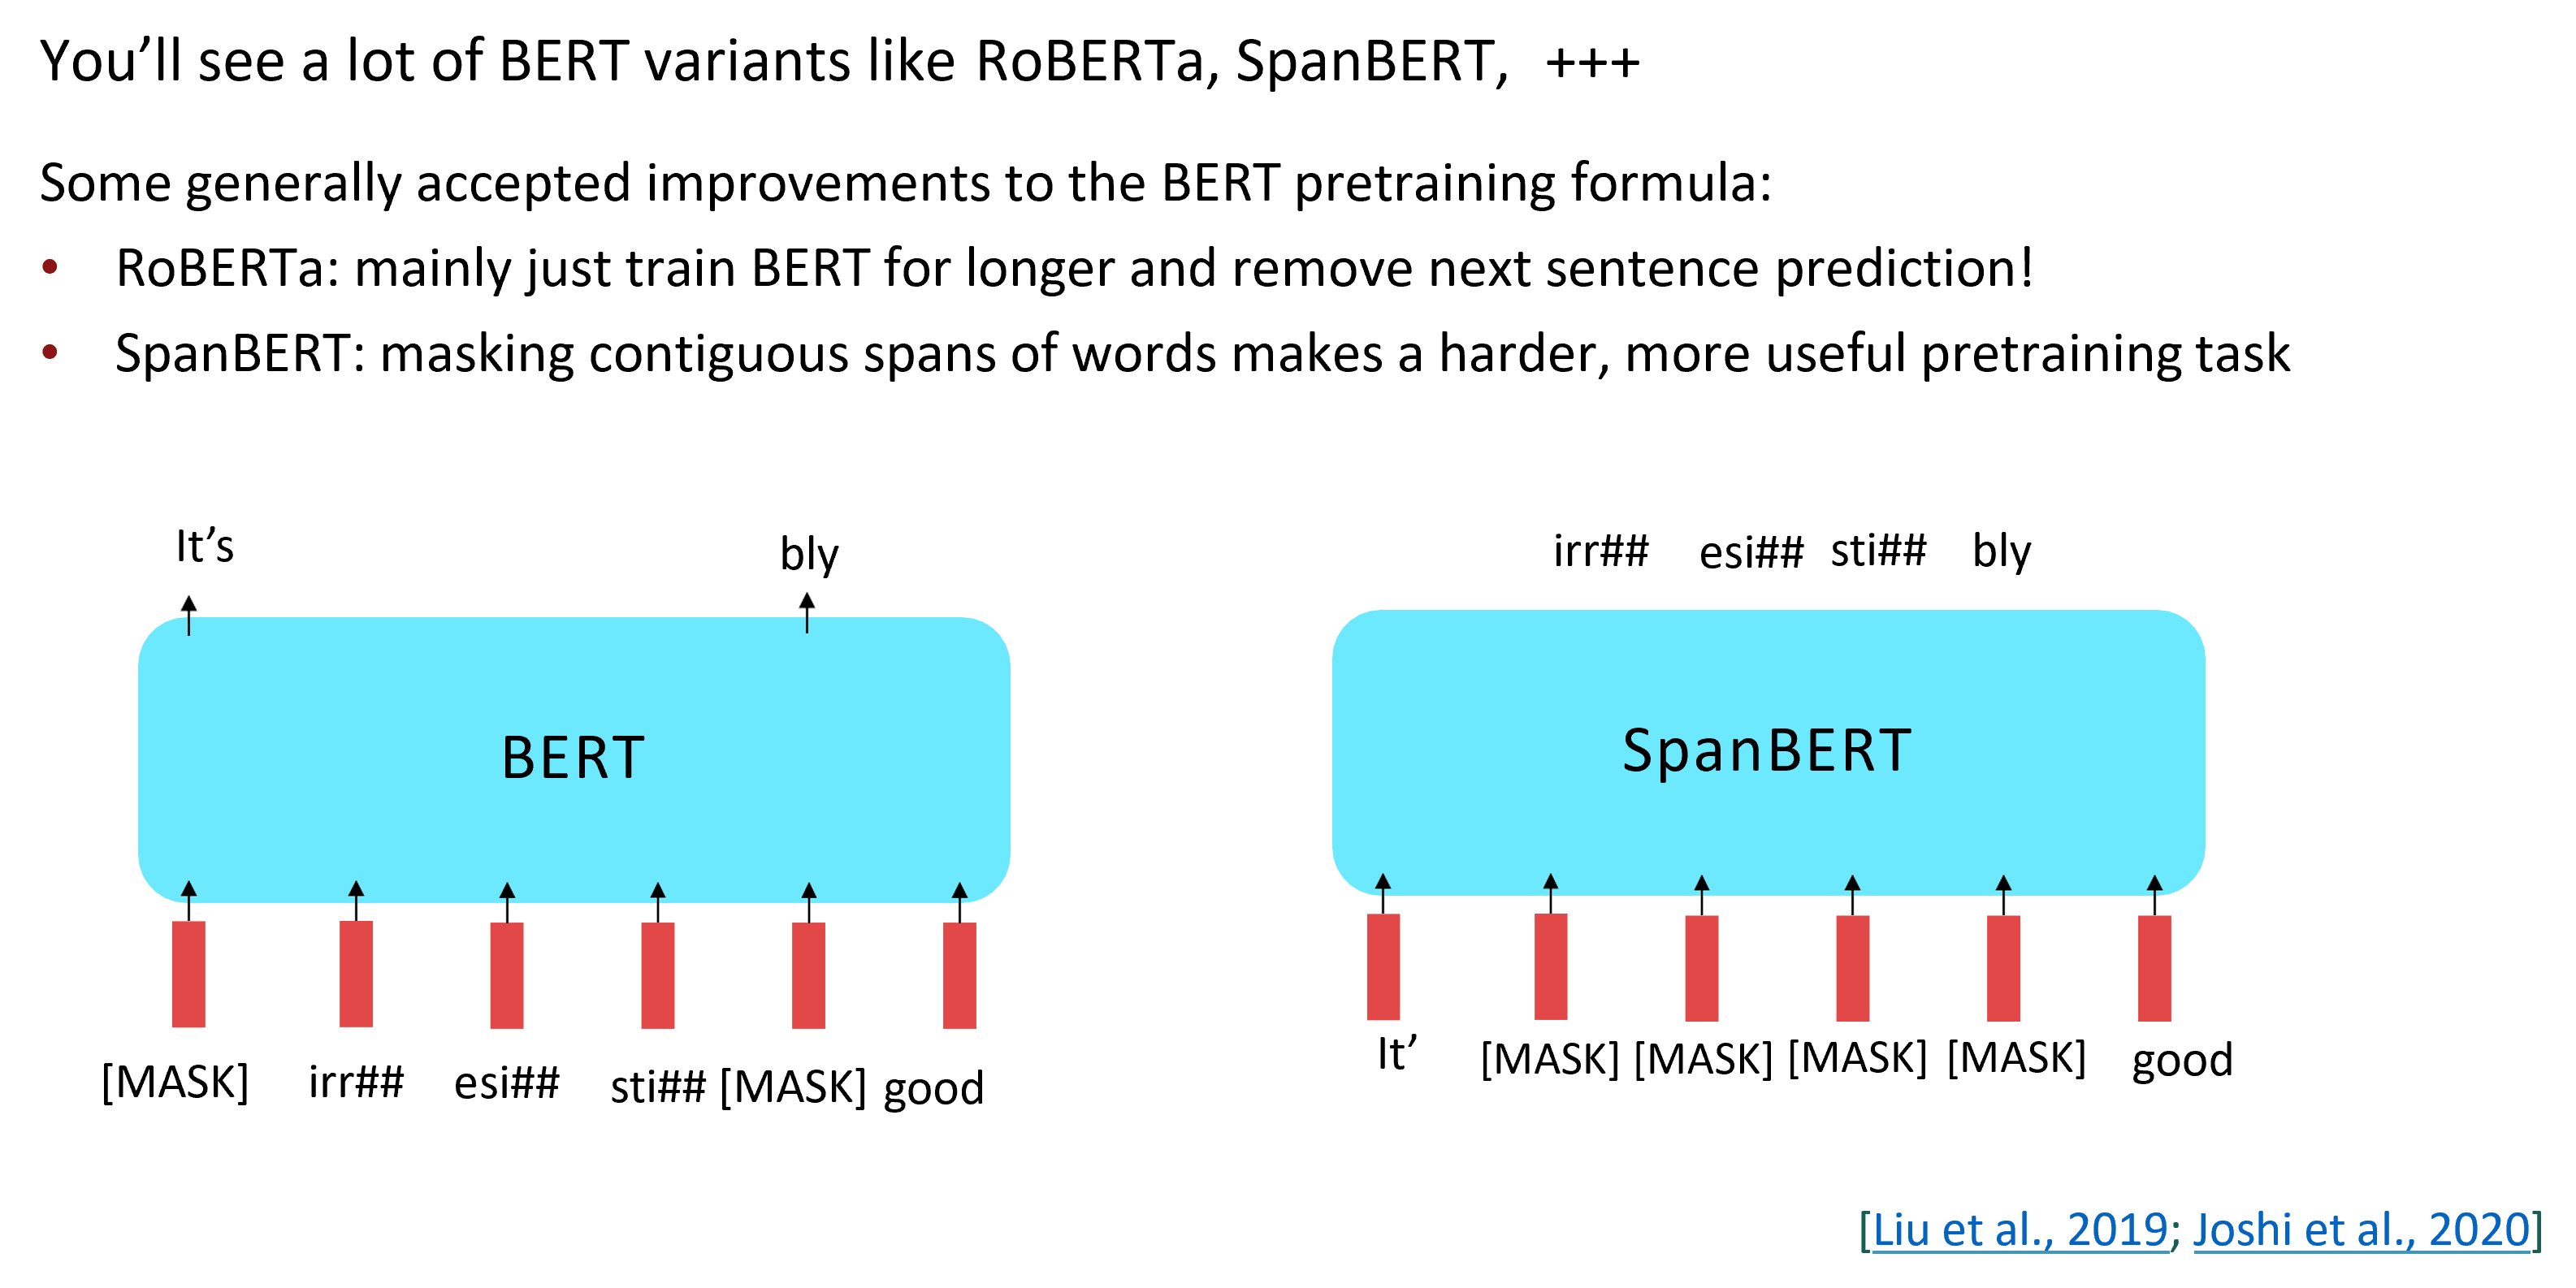
\includegraphics[width=\linewidth,keepaspectratio]{bert124}
			\end{center}		
			
			% {\tiny (Ref: John Hewitt)}

\end{frame}

%%%%%%%%%%%%%%%%%%%%%%%%%%%%%%%%%%%%%%%%%%%%%%%%%%%%%%%%%%%
\begin{frame}[fragile]\frametitle{Input}

		\begin{itemize}
		\item Use 30,000 WordPiece vocabulary on input. 
		\item Each token is sum of three embeddings 
		\item Single sequence is much more efficient
		\end{itemize}


			\begin{center}
			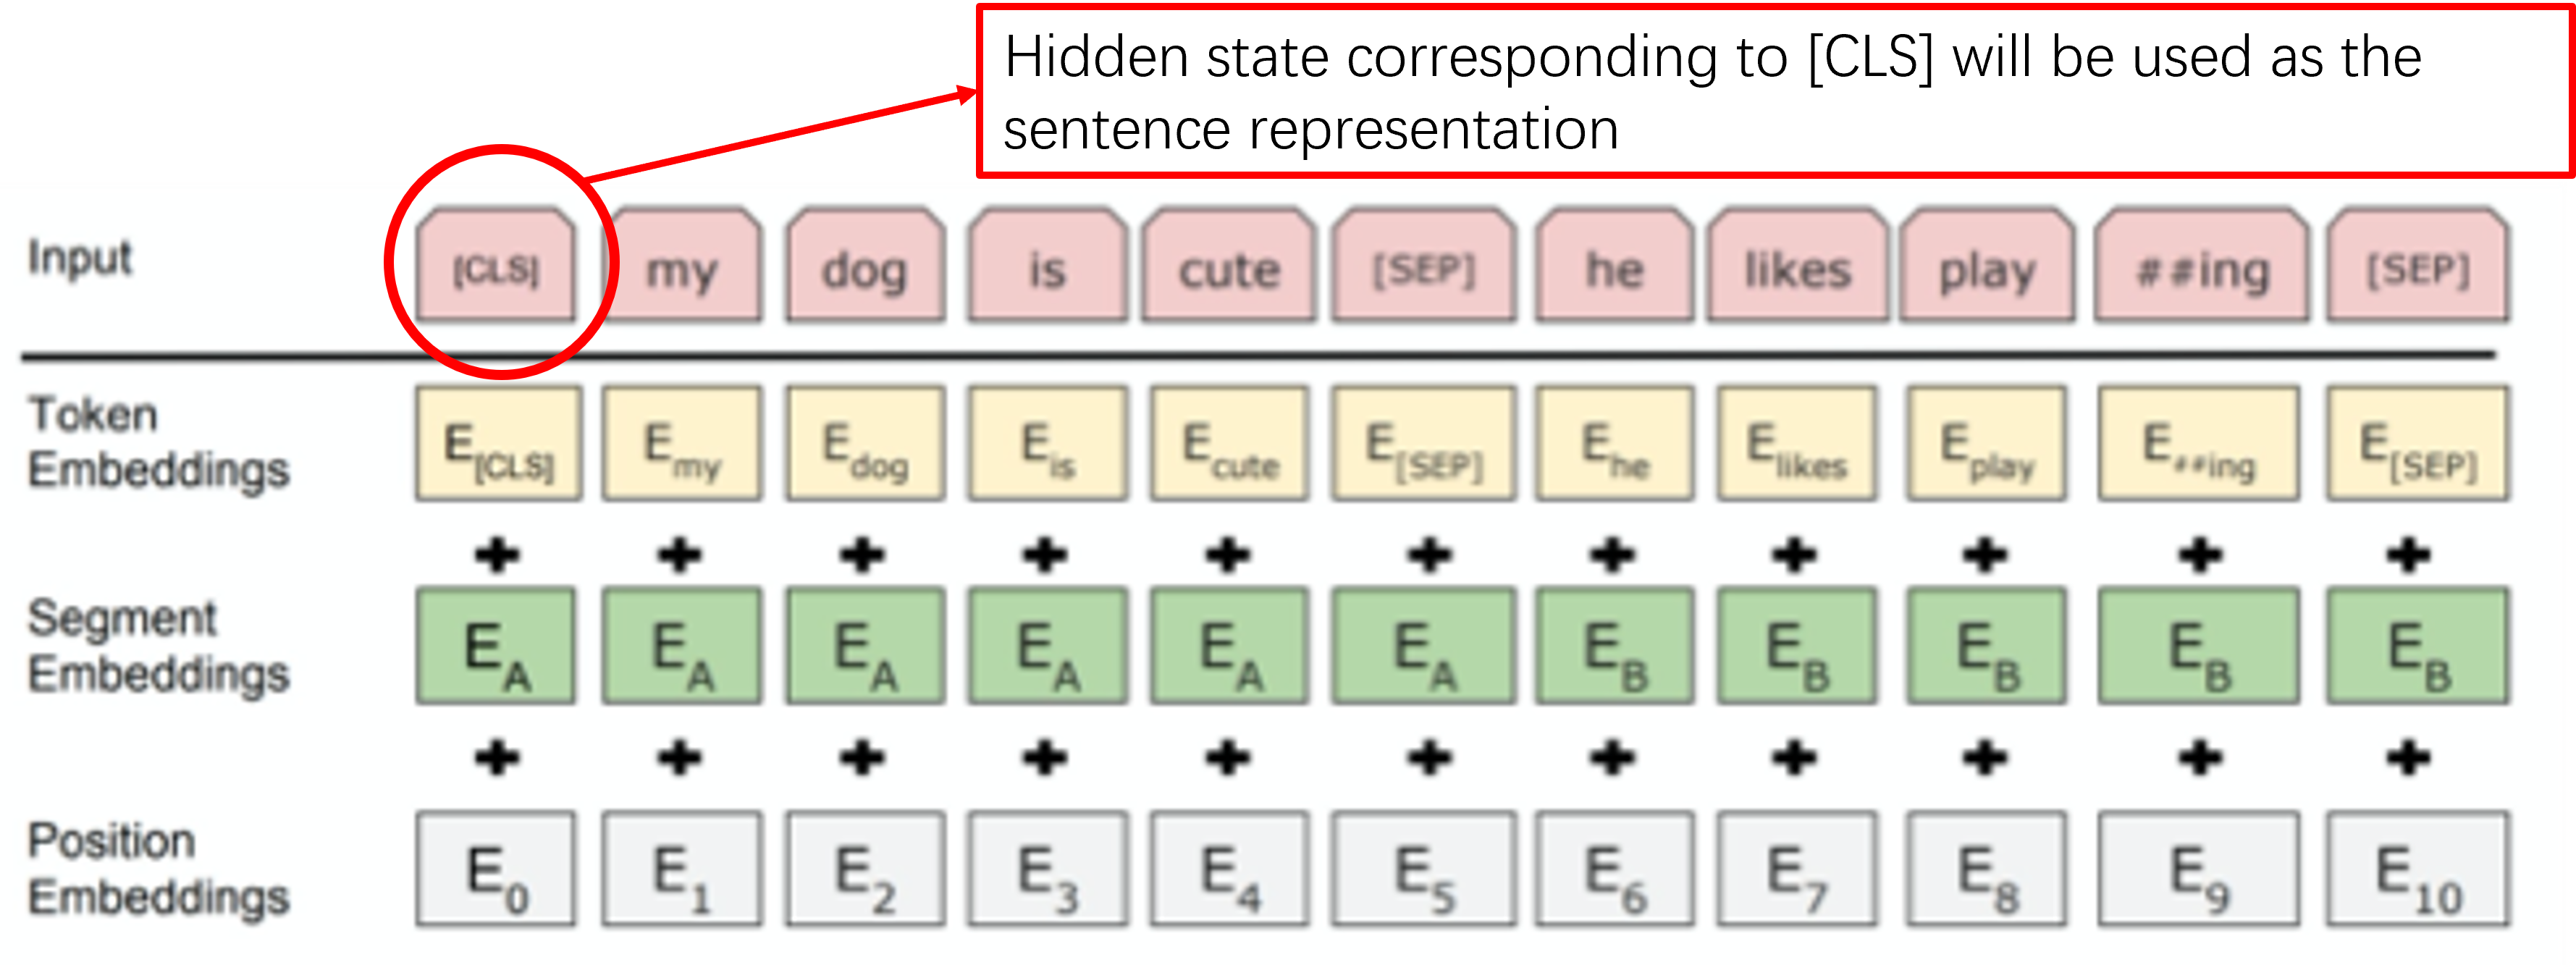
\includegraphics[width=\linewidth,keepaspectratio]{bert125}
			\end{center}		
			

\end{frame}

%%%%%%%%%%%%%%%%%%%%%%%%%%%%%%%%%%%%%%%%%%%%%%%%%%%%%%%%%%%
\begin{frame}[fragile]\frametitle{WordPiece (Tokenizer)}

		\begin{itemize}
		\item BERT uses a variant of the wordpiece model
		\item Given a training corpus and a number of desired tokens D, select D wordpieces such that the resulting corpus is minimal in the number of wordpieces when segmented according to the chosen wordpiece model. 
		\item wordpieces give a good balance between the flexibility of single characters and the efficiency of full words for decoding, and also sidesteps the need for special treatment of unknown words.
		\item Examples:
				\begin{itemize}

		\item Common words which are in vocabulary: ‘at’, ‘Fairfax’, ‘1910s’
		\item Uncommon words are built using wordpieces: ‘Hypatia’ = h \#\#yp \#\#ati \#\#a
		\end{itemize}

		\end{itemize}

		

\end{frame}

%%%%%%%%%%%%%%%%%%%%%%%%%%%%%%%%%%%%%%%%%%%%%%%%%%%%%%%%%%%
\begin{frame}[fragile]\frametitle{Tokenizer}

			\begin{center}
			
\includegraphics[width=\linewidth,keepaspectratio]{bert126}
			\end{center}	

\end{frame}

%%%%%%%%%%%%%%%%%%%%%%%%%%%%%%%%%%%%%%%%%%%%%%%%%%%%%%%%%%%
\begin{frame}[fragile]\frametitle{ Unidirectional vs. Bidirectional Models}

			\begin{center}
			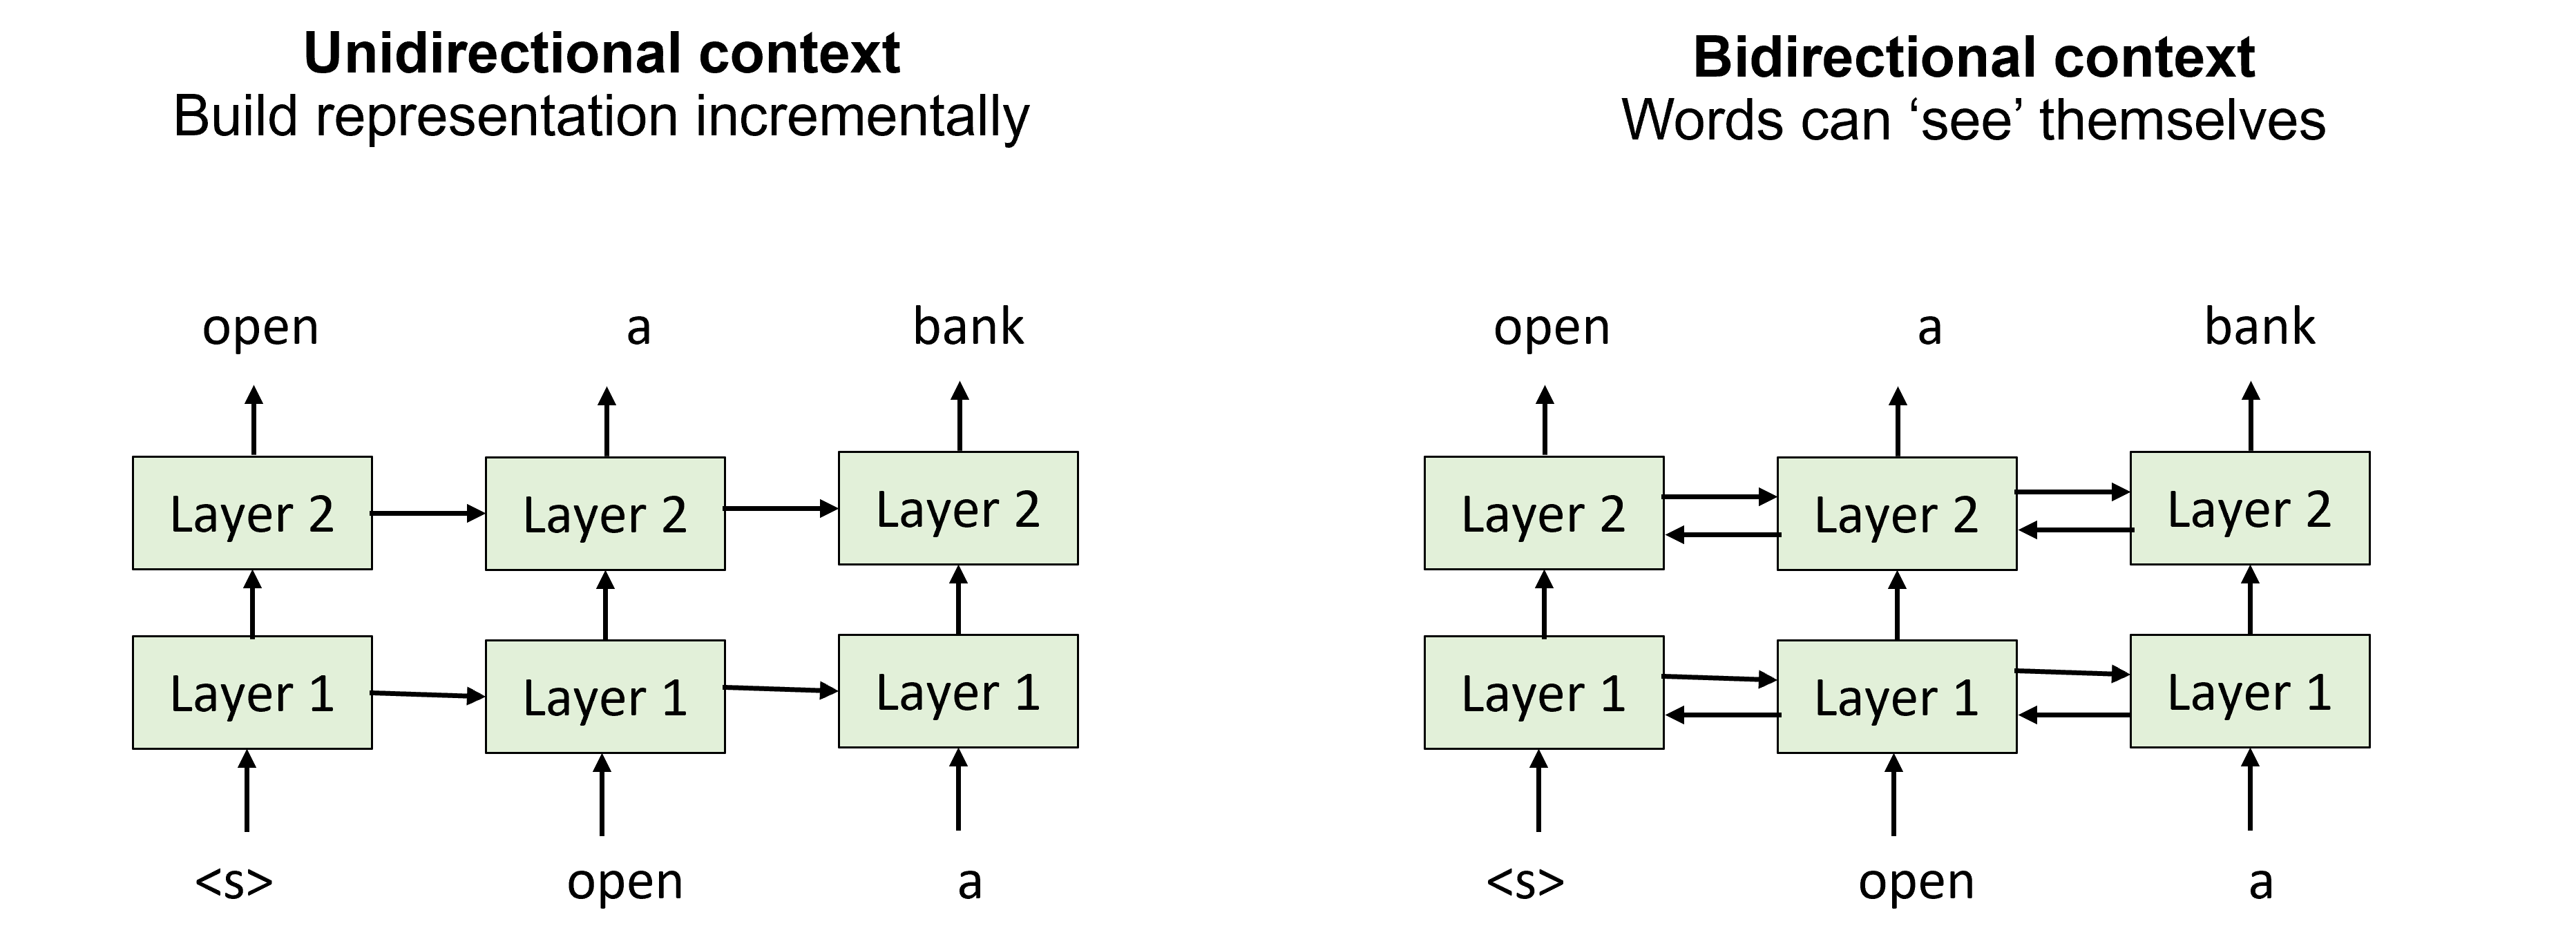
\includegraphics[width=\linewidth,keepaspectratio]{bert127}
			\end{center}	

\end{frame}

%%%%%%%%%%%%%%%%%%%%%%%%%%%%%%%%%%%%%%%%%%%%%%%%%%%%%%%%%%%
\begin{frame}[fragile]\frametitle{ BERT Training}

			\begin{center}
			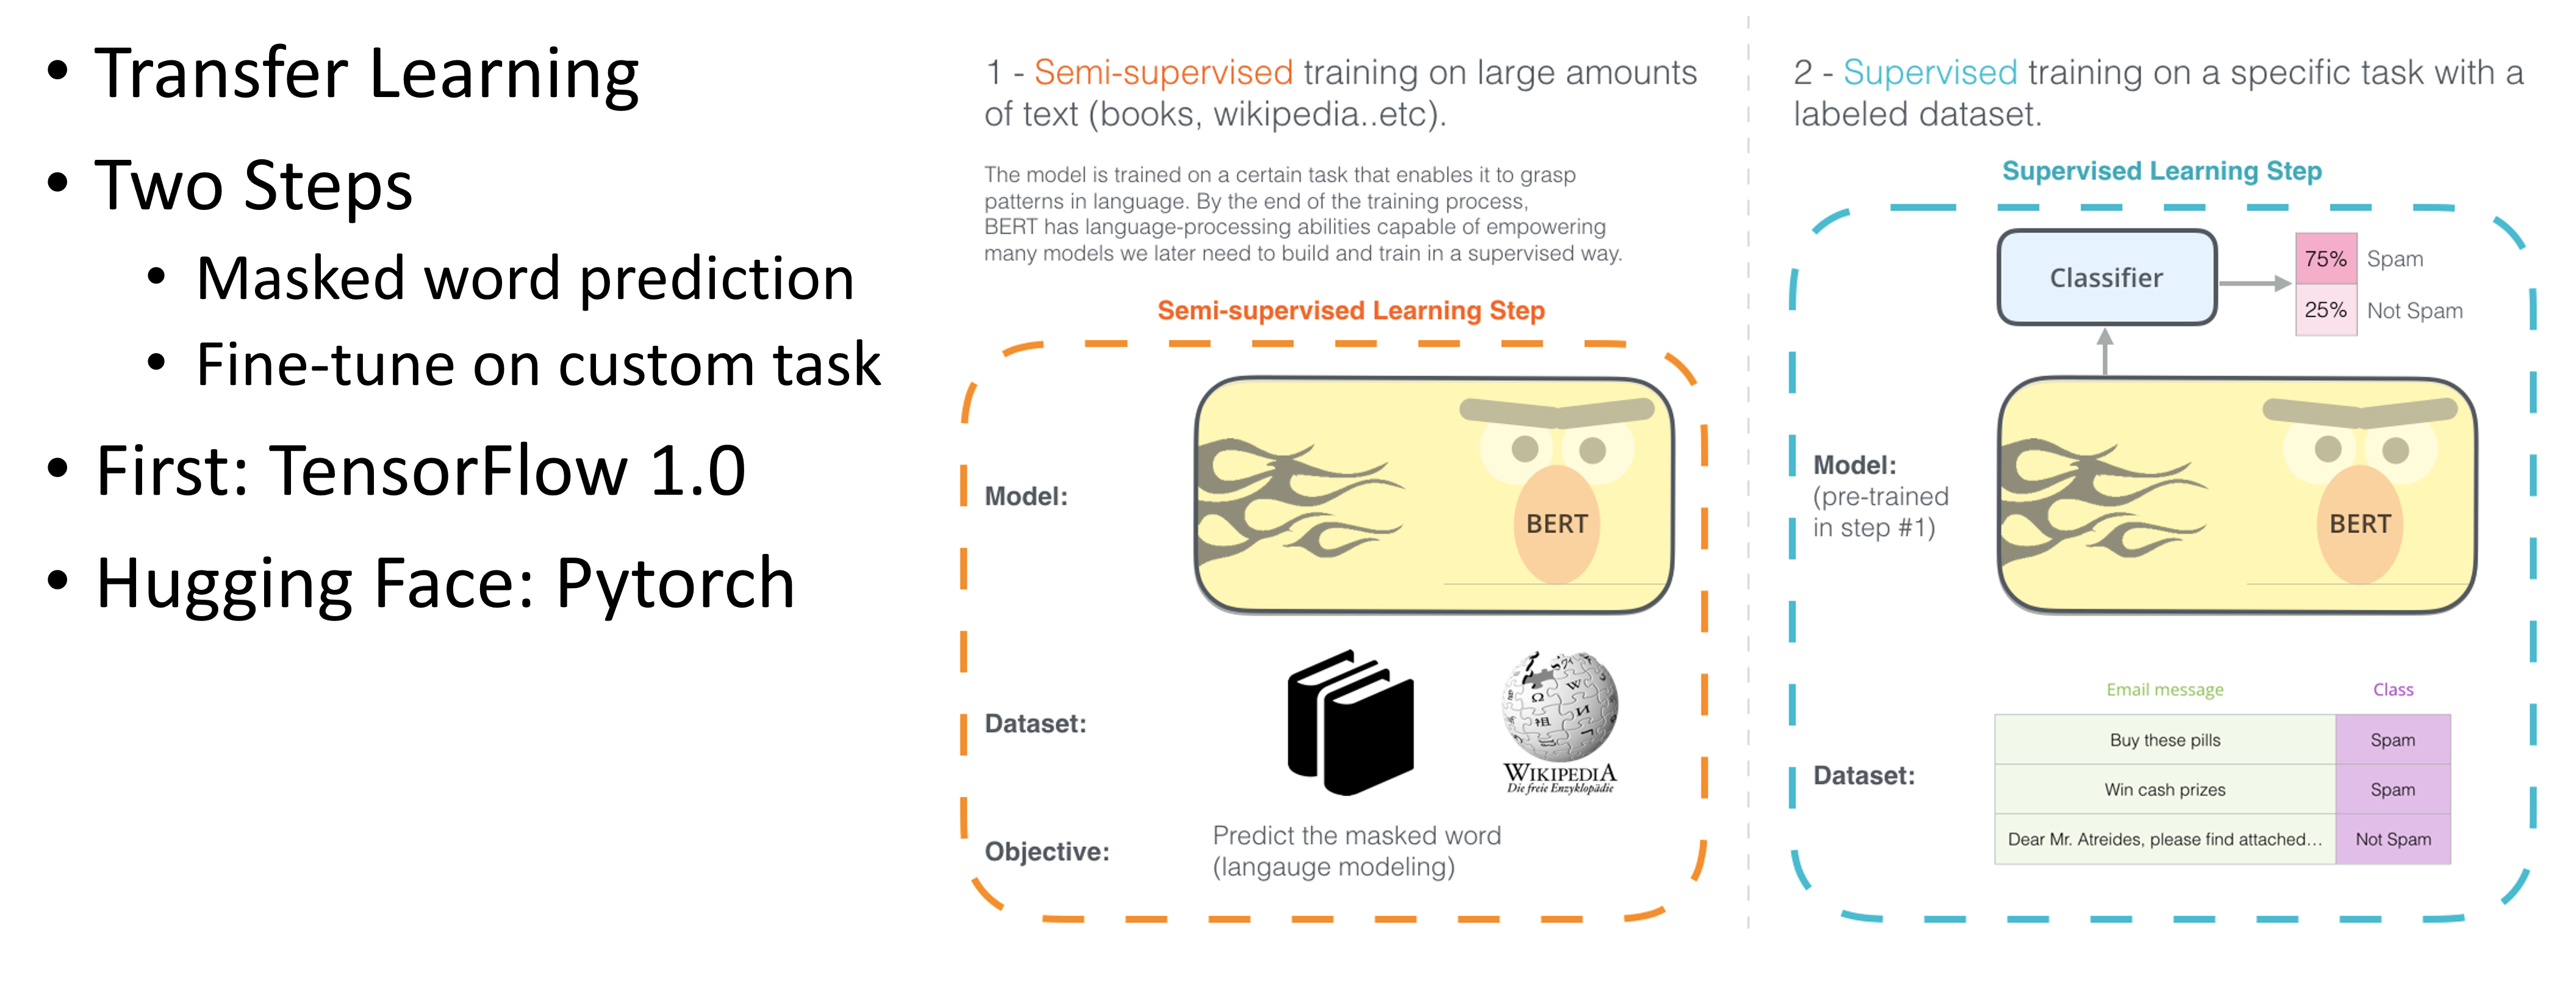
\includegraphics[width=\linewidth,keepaspectratio]{bert128}
			\end{center}	

% {\tiny (Ref: The Illustrated BERT, ELMo, and co. (How NLP Cracked Transfer Learning) – Jay Alammar)}

\end{frame}

%%%%%%%%%%%%%%%%%%%%%%%%%%%%%%%%%%%%%%%%%%%%%%%%%%%%%%%%%%%
\begin{frame}[fragile]\frametitle{Pre-Training}

			\begin{center}
			
\includegraphics[width=\linewidth,keepaspectratio]{bert129}
			\end{center}	


\end{frame}
